\chapter{测地线、均匀加速度与牛顿极限}

直接的问题是引力。更确切地说，我们想要描述近乎均匀引力场的时空度规，例如地球表面附近一个小实验室中的场。通向该度规的最短路径结果并非一条直接的路径。我们必须首先使三个几何概念变得可操作：协变微分、平行移动和测地运动。

这些概念彼此依赖。协变微分告诉我们如何比较相邻点处的矢量。平行移动告诉我们如何在不转动矢量的情况下搬运它。当被搬运的矢量是路径自身的切矢量时，就得到一条测地线。一旦路径位于时空中而非空间中，同一个测地线方程就成为自由下落粒子的运动方程。

讲座的后半部分随后做出一个引人注目的举动。我们仍停留在平坦的闵可夫斯基时空中，但用适应于一个刚性加速观察者族的坐标来描述它。在这些坐标中，度规看起来像引力。在一个观察者附近，它再现了均匀场的势，并且其测地线服从牛顿方程
\begin{equation}
\frac{d^2y}{d\tau^2}=-g.
\end{equation}
这就是写成计算的等效原理。

\section{协变导数的回顾}

在选定的点\(P\)处，可以选择尽可能笛卡儿的坐标。讲座最初使用高斯法坐标这一说法，然后立即对其加以限定。名称不如局部条件重要：
\begin{equation}
g_{mn}(P)=\delta_{mn},
\qquad
\partial_r g_{mn}(P)=0.
\label{eq:l4-normal-point}
\end{equation}
这些是在一个点处的法坐标。它们不必在有限邻域内保持笛卡儿，并且存在许多这样的标架，因为其轴可以旋转。

度规与导数算符相容：
\begin{equation}
\nabla_r g_{mn}=0,
\qquad
\nabla_r g^{mn}=0.
\label{eq:l4-metric-compatibility}
\end{equation}
对于余矢量\(V_s\)，协变导数为
\begin{equation}
\nabla_r V_s
=
\partial_r V_s-\Gamma^p{}_{rs}V_p.
\label{eq:l4-covector-derivative}
\end{equation}
联络系数为
\begin{equation}
\Gamma^p{}_{rs}
=
\frac{1}{2}g^{pn}
\left(
\partial_s g_{nr}
+\partial_r g_{ns}
-\partial_n g_{rs}
\right).
\label{eq:l4-christoffel}
\end{equation}
当这个表达式写在黑板上时，若干指标被更正。方程\eqref{eq:l4-christoffel}是完成后的关系。它在\(r\)和\(s\)中是对称的，正如无挠列维-奇维塔联络所预期的那样。

\begin{figure}[htbp]
\centering
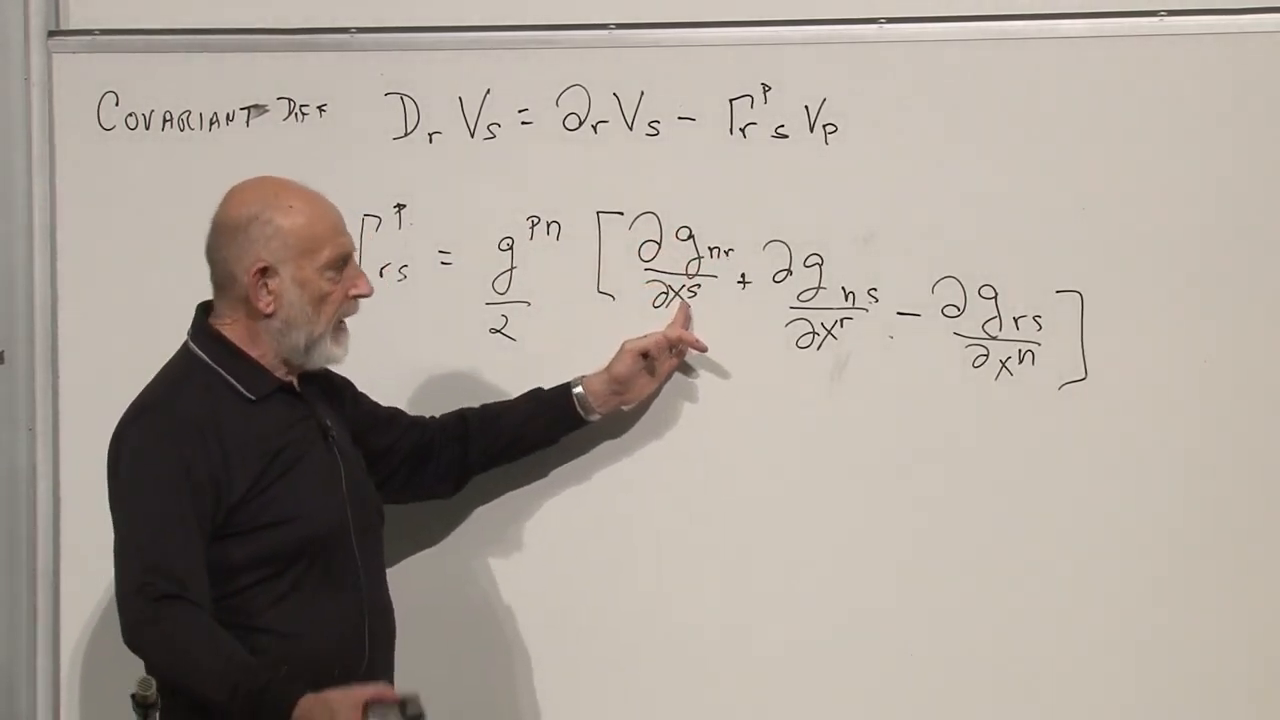
\includegraphics[width=0.92\textwidth]{lecture_04_figure_01.png}
\caption{余矢量导数与完成后的克里斯托费尔符号公式。}
\end{figure}

因为克里斯托费尔符号由度规的一阶导数构成，所以在坐标\eqref{eq:l4-normal-point}中它们在\(P\)处为零。即使底空间是平坦的，它们也并非在每个坐标系中都为零。因此\(\Gamma^p{}_{rs}\)不是张量。这种非张量特性后来恰恰使得加速观察者能够描述一种惯性观察者看不到的引力。

\subsection{提升矢量指标}

矢量的相应导数不是作为一条单独规则引入来记忆的。它由度规推出。从
\begin{equation}
V^n=g^{np}V_p.
\end{equation}
开始，然后
\begin{align}
\nabla_m V^n
&=\nabla_m\!\left(g^{np}V_p\right) \\
&=(\nabla_m g^{np})V_p+g^{np}\nabla_m V_p \\
&=g^{np}\left(\partial_mV_p-\Gamma^r{}_{mp}V_r\right),
\end{align}
其中度规相容性去掉了第一项。重新整理指标得到
\begin{equation}
\nabla_m V^n
=
\partial_m V^n+\Gamma^n{}_{mr}V^r.
\label{eq:l4-vector-derivative}
\end{equation}

\begin{figure}[htbp]
\centering
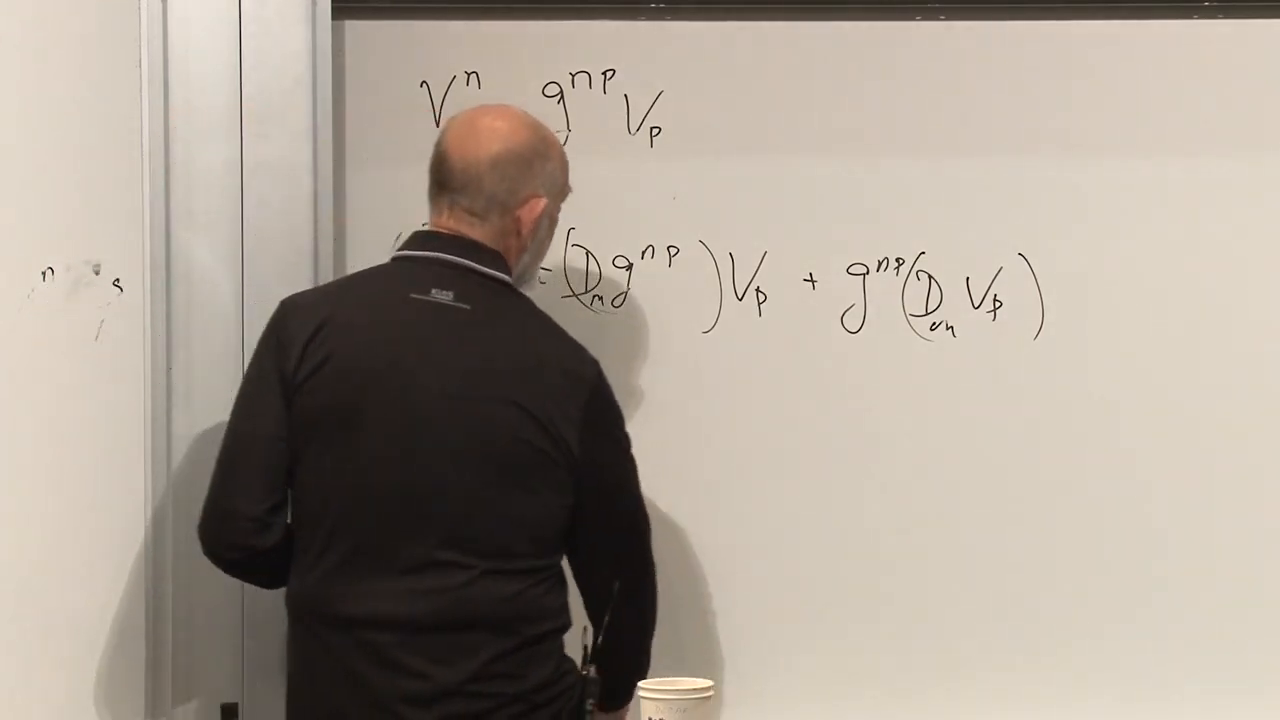
\includegraphics[width=0.90\textwidth]{lecture_04_figure_02.png}
\caption{在微分之前用逆度规提升指标。}
\end{figure}

\begin{figure}[htbp]
\centering
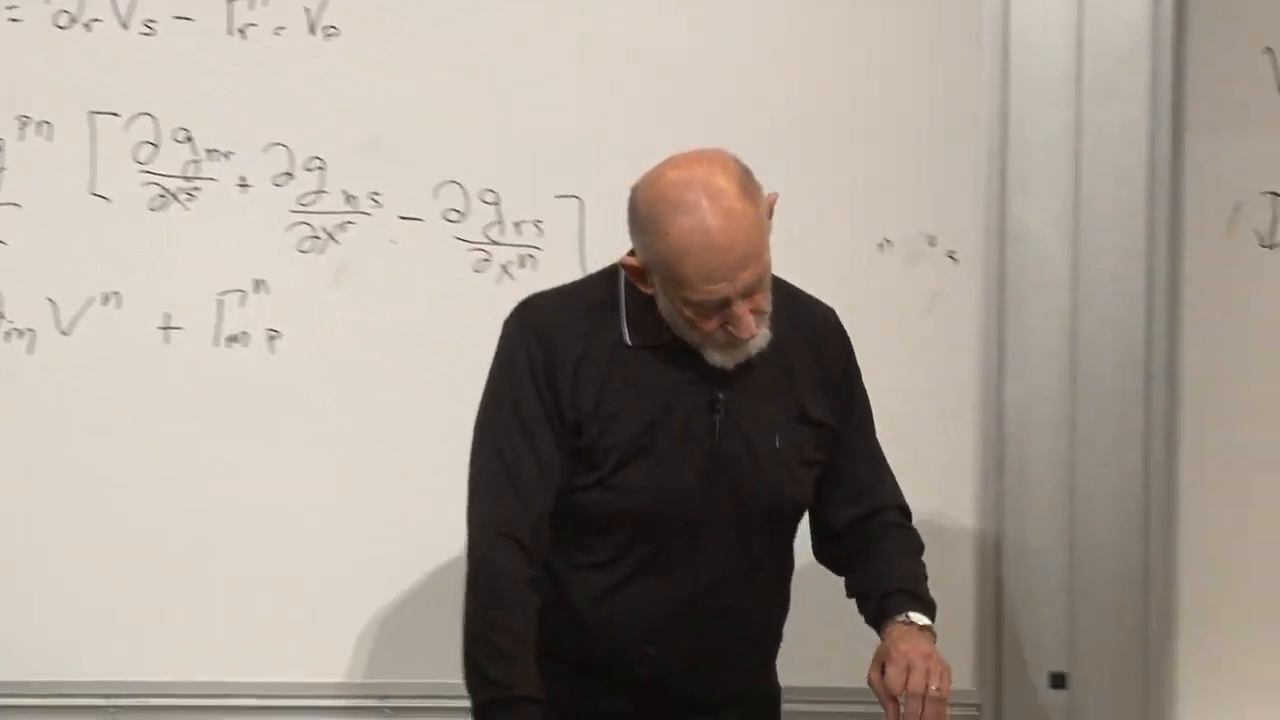
\includegraphics[width=0.90\textwidth]{lecture_04_figure_03.png}
\caption{由度规相容性和乘积法则得出的上指标导数。}
\end{figure}

因此指标语法很简单：
\begin{equation}
\boxed{
\begin{aligned}
\text{lower index:}&\quad -\Gamma,\\
\text{upper index:}&\quad +\Gamma.
\end{aligned}}
\end{equation}
对于更高阶的张量，每个指标出现一个联络项，其符号由该指标是下指标还是上指标决定。

\subsection{一个术语问题}

上面提到的最佳坐标究竟是什么？它们并未被断言为一个特殊的全局坐标系。在一个选定的点处，它们使度规等于其平坦形式，并使其一阶导数为零。旋转坐标轴会给出另一个同样好的标架。在这样的标架中导出的几何陈述不依赖于该取向，因为最终的客体是张量。

\section{沿曲线的平行移动}

假设一个矢量\(V^n\)沿一条曲线被搬运。在无穷小位移\(dx^m\)上，其协变变化为
\begin{align}
\delta V^n
&=(\nabla_mV^n)\,dx^m \\
&=\partial_mV^n\,dx^m
+\Gamma^n{}_{mr}V^r\,dx^m \\
&=dV^n+\Gamma^n{}_{mr}V^r\,dx^m.
\label{eq:l4-covariant-differential}
\end{align}

\begin{figure}[htbp]
\centering
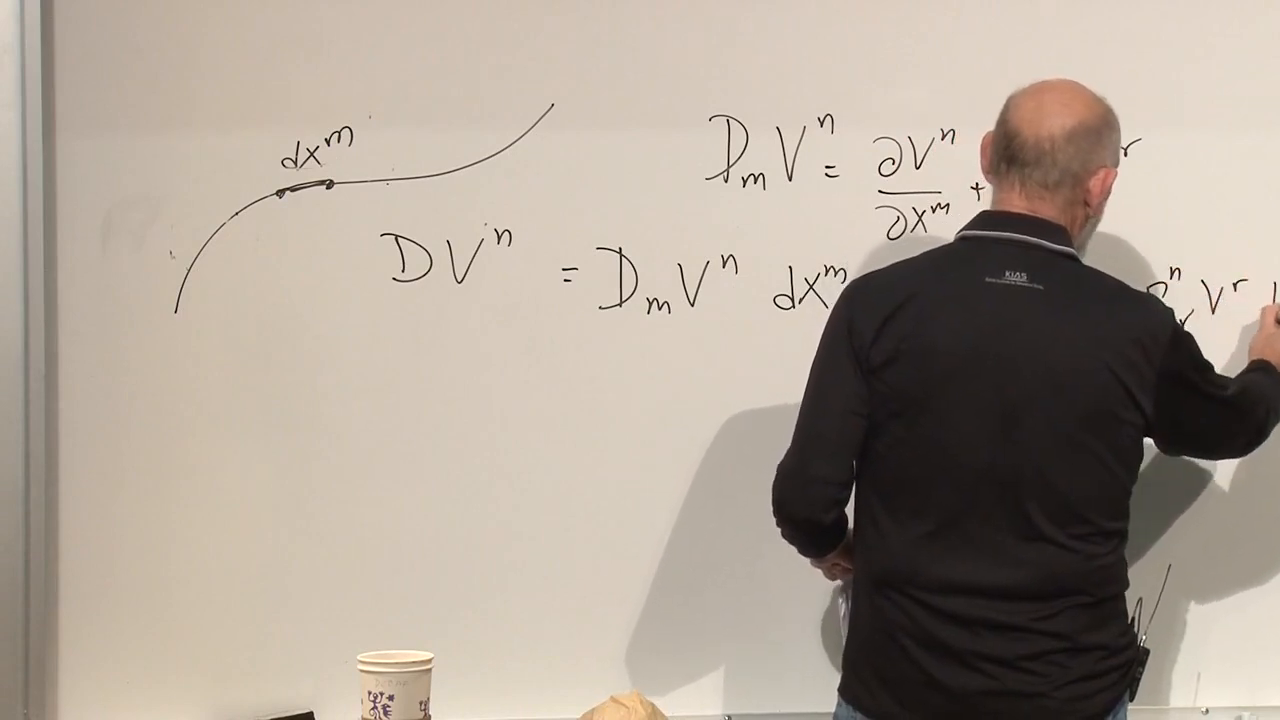
\includegraphics[width=0.92\textwidth]{lecture_04_figure_04.png}
\caption{沿曲线的普通分量变化与联络修正。}
\end{figure}

当这个协变变化为零时，矢量被平行移动：
\begin{equation}
\boxed{
dV^n+\Gamma^n{}_{mr}V^r\,dx^m=0.
}
\label{eq:l4-parallel-transport}
\end{equation}
在操作上，我们可以想象在曲线的每一点处建立一个法标架。在那个局部标架中，要求被搬运的矢量不转动。然后我们移动一个无穷小距离，建立下一个法标架，并重复。

\begin{figure}[htbp]
\centering
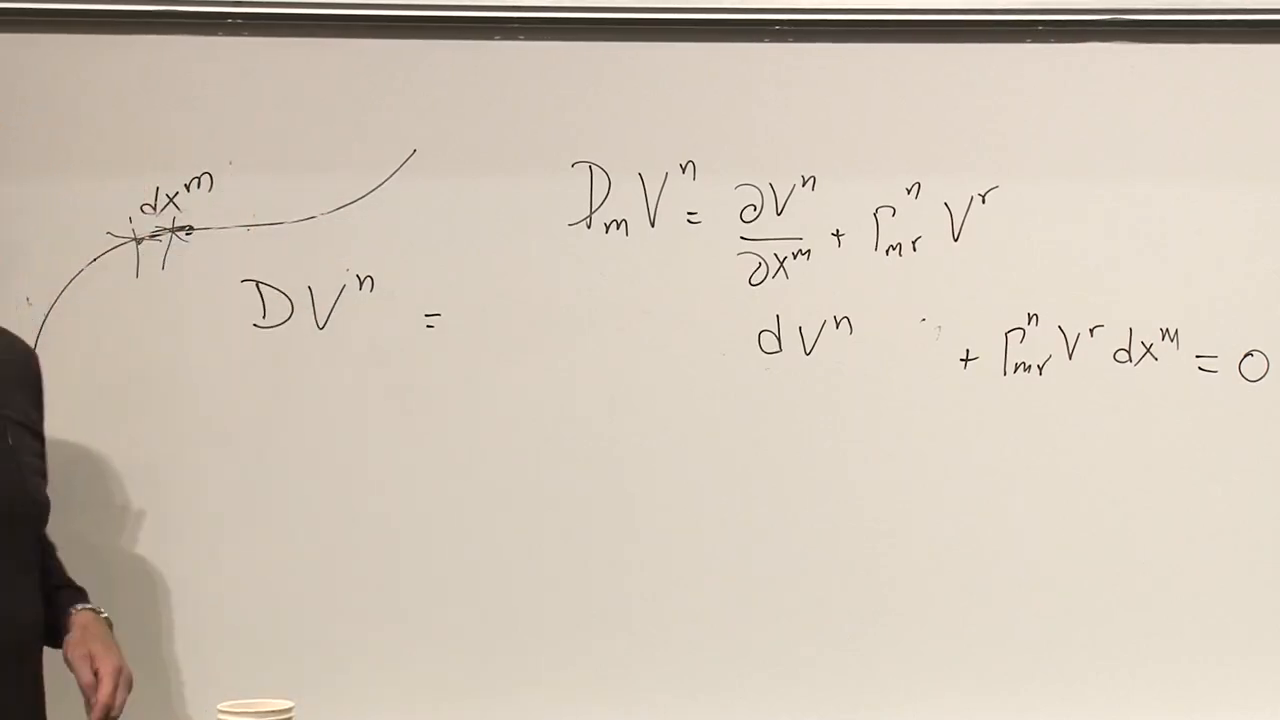
\includegraphics[width=0.92\textwidth]{lecture_04_figure_05.png}
\caption{平行移动方程的一个清晰黑板状态。}
\end{figure}

每个临时正交标架的取向并不属于物理内容。我们可以在进行比较之前旋转它。真正重要的是，协变陈述\eqref{eq:l4-parallel-transport}与这一任意选择无关。

\subsection{路径依赖与曲率}

在弯曲空间中，平行移动依赖于路径。从同一初始点上的同一矢量出发，沿两条不同路线将它移动到同一终点。一般而言，最终的矢量不同。让一个矢量沿闭合回路移动，返回时它可能已被旋转。这种不匹配就是和乐，它是曲率的直接标志。

\begin{figure}[htbp]
\centering
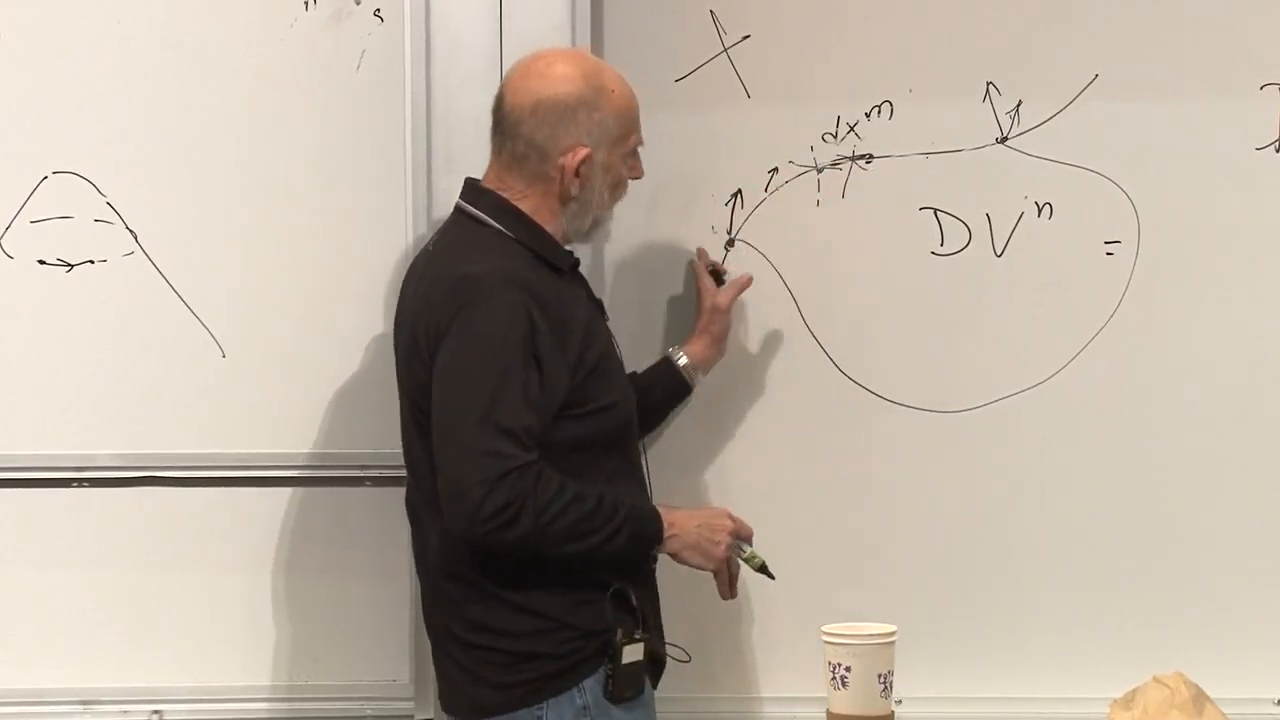
\includegraphics[width=0.90\textwidth]{lecture_04_figure_06.png}
\caption{弯曲曲面上的两条路线未必把矢量平行移动到相同的最终取向。}
\end{figure}

圆锥提供了一个有用的例子。在远离其顶点处，圆锥可以剪开并展平。然而，沿一条包围顶点的回路进行平行移动，返回时矢量会被角度亏损所旋转。如果顶点被磨圆，曲率就是有限的，并分布在一个小区域上。如果顶点完全尖锐，这种理想化就把曲率集中在顶点处。

\begin{figure}[htbp]
\centering
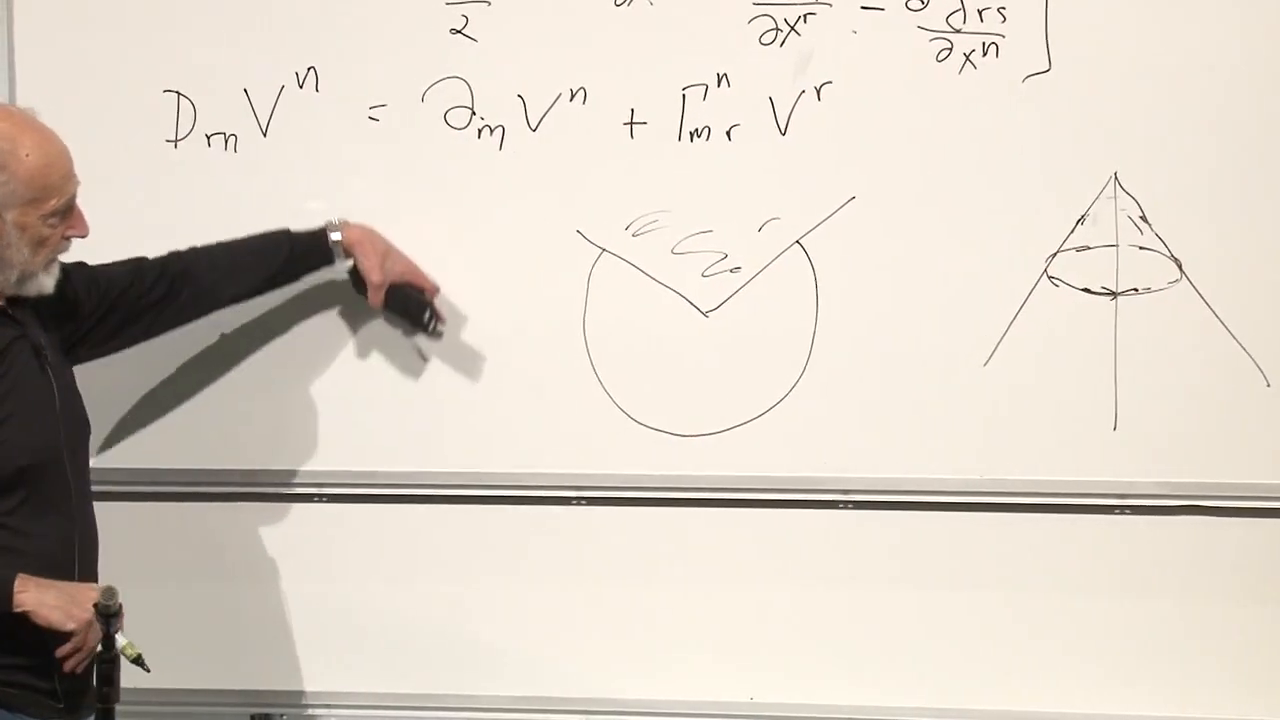
\includegraphics[width=0.90\textwidth]{lecture_04_figure_07.png}
\caption{圆锥上的圆周运动及其剪开展平的平面表示。}
\end{figure}

\subsection{关于被移动矢量的问题}

\paragraph{矢量必须在处处都有定义吗？}
不。可以从一点上的单个矢量出发，只沿所选曲线求解\eqref{eq:l4-parallel-transport}。完整的矢量场是可选的。如果已经在一个区域上定义了场，它可能沿一个方向协变常定，而沿另一个方向则不是。

\paragraph{它的长度保持不变吗？}
是的。令\(V^2=g_{mn}V^mV^n\)。沿曲线，
\begin{align}
\frac{D}{d\lambda}\left(g_{mn}V^mV^n\right)
&=
\frac{Dg_{mn}}{d\lambda}V^mV^n
+2g_{mn}V^m\frac{DV^n}{d\lambda}\\
&=0.
\end{align}
度规相容性消去第一项，平行移动消去第二项。因此，平行移动矢量的长度与相互夹角都保持不变。

\paragraph{每条曲线的切矢量都平行移动吗？}
不。这个问题直接引向测地线。绕圆锥的圆形路线的切矢量不断转向。把圆锥剪开展平后所得直线的切矢量则不转向。只有第二条路径是局部笔直的。

\section{测地线：最直而非仅仅最短}

测地线有两种相关的描述。整体上，它是长度或固有时泛函的驻定路径。局部上，它是尽可能最直的路径。驻定一词很重要：取决于几何与端点，这条路径未必是唯一的整体最小值。在洛伦兹时空中，类时测地线局部上使固有时最大，而不是使某个正距离最小。

这里需要的是局部描述。一辆小汽车在弯曲地形上行驶，方向盘保持正前方，就会描出一条测地线，只要汽车相比地形弯曲的尺度足够小。它在嵌入空间中未必看起来是直的；按照曲面上可用的几何，它是直的。

\begin{figure}[htbp]
\centering
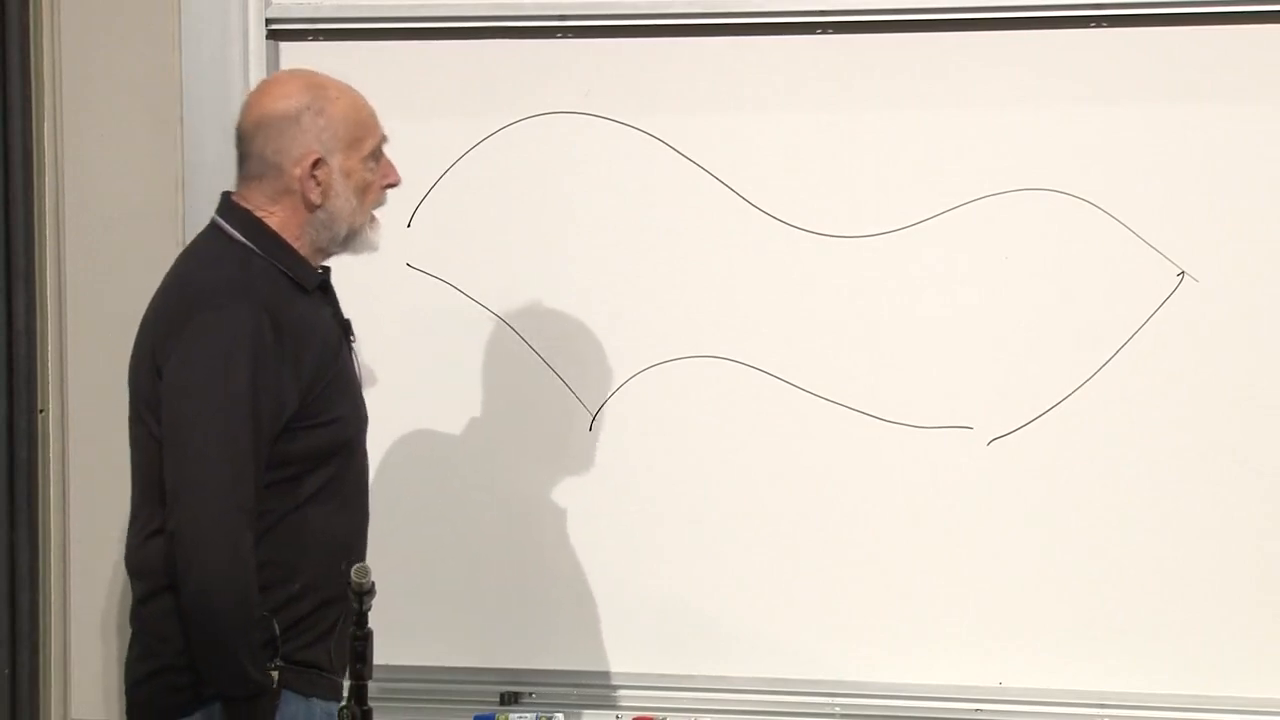
\includegraphics[width=0.90\textwidth]{lecture_04_figure_08.png}
\caption{在弯曲曲面上内蕴地画出的一条路径，为最直路径的定义作准备。}
\end{figure}

\subsection{切矢量}

设曲线为\(x^m(s)\)，其弧长为
\begin{equation}
ds^2=g_{mn}\,dx^m dx^n.
\end{equation}
单位切矢量为
\begin{equation}
t^m=\frac{dx^m}{ds}.
\label{eq:l4-unit-tangent}
\end{equation}
几何上，取两个邻近点，构造它们之间的位移矢量，除以它们的间隔，再让这两点合并。

\begin{figure}[htbp]
\centering
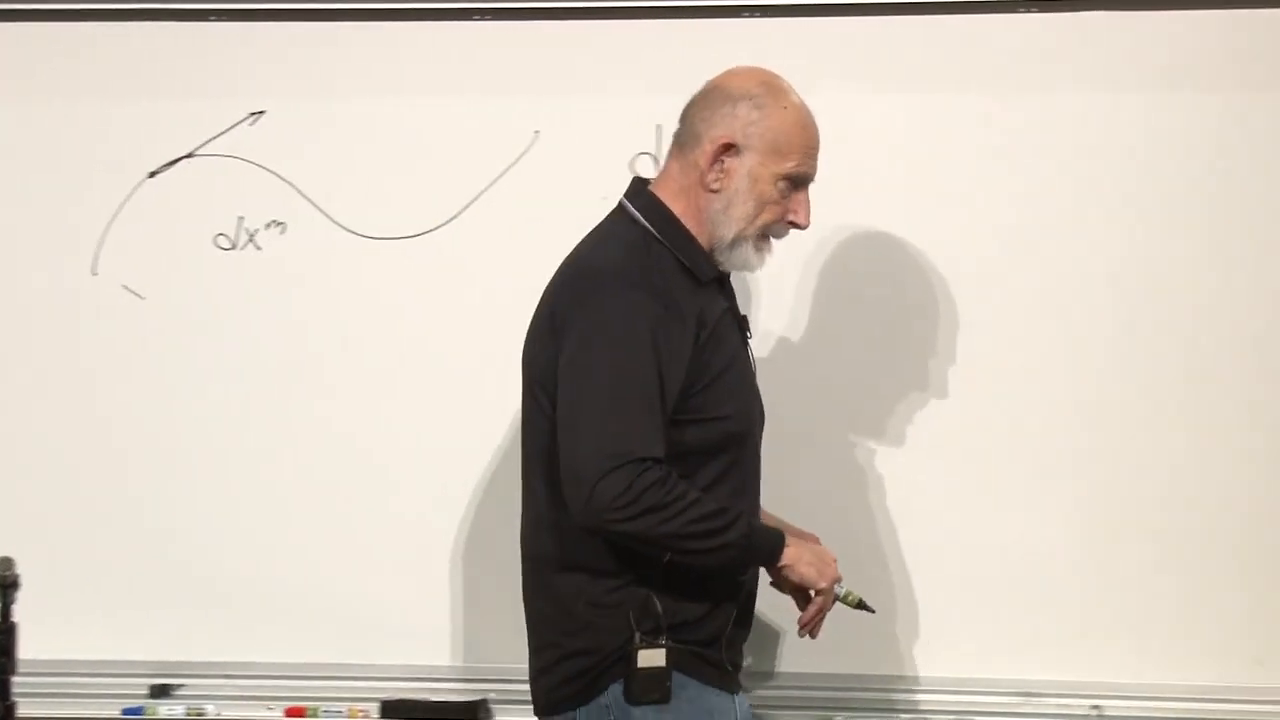
\includegraphics[width=0.90\textwidth]{lecture_04_figure_09.png}
\caption{切方向作为沿曲线的极限位移。}
\end{figure}

\begin{figure}[htbp]
\centering
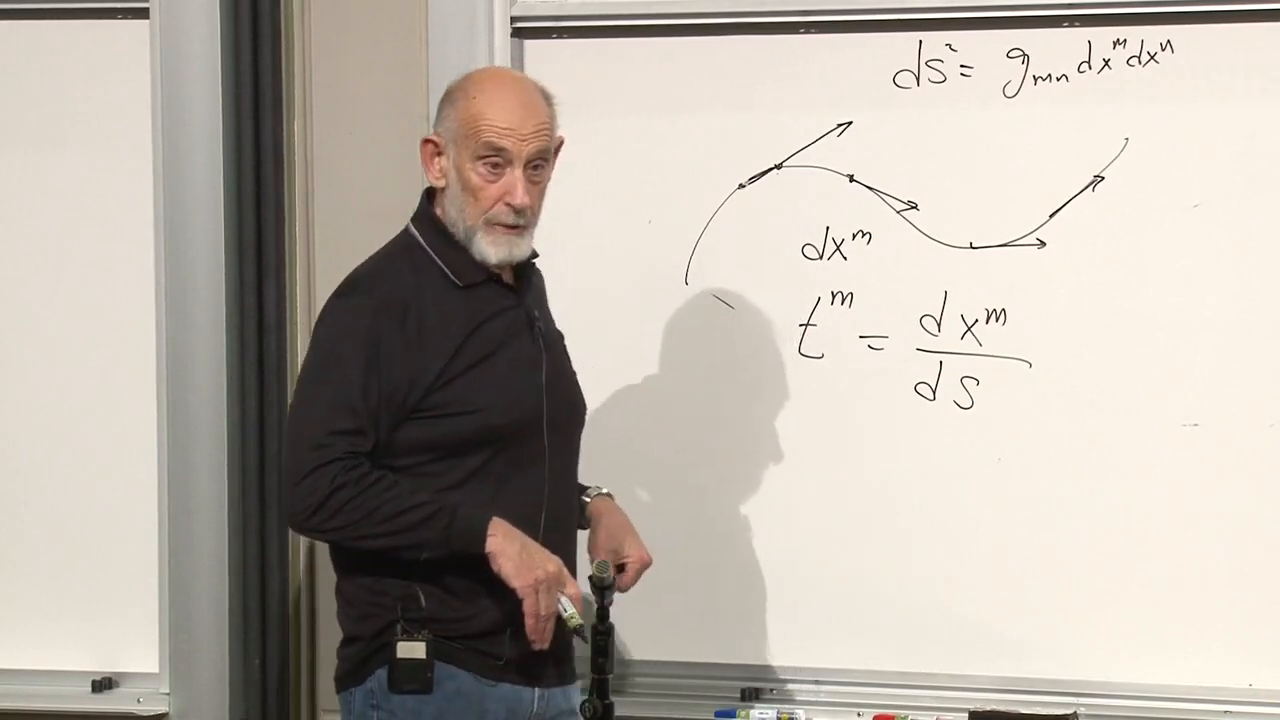
\includegraphics[width=0.90\textwidth]{lecture_04_figure_10.png}
\caption{线元与单位切矢量\(t^m=dx^m/ds\)。}
\end{figure}

测地线是其切矢量沿自身平行移动的曲线：
\begin{equation}
dt^n+\Gamma^n{}_{mr}t^r\,dx^m=0.
\end{equation}
除以\(ds\)并使用\(dx^m/ds=t^m\)：
\begin{equation}
\frac{dt^n}{ds}
=
-\Gamma^n{}_{mr}t^m t^r.
\end{equation}
最后代入\(t^n=dx^n/ds\)：
\begin{equation}
\boxed{
\frac{d^2x^n}{ds^2}
+\Gamma^n{}_{mr}
\frac{dx^m}{ds}
\frac{dx^r}{ds}
=0.
}
\label{eq:l4-geodesic}
\end{equation}

\begin{figure}[htbp]
\centering
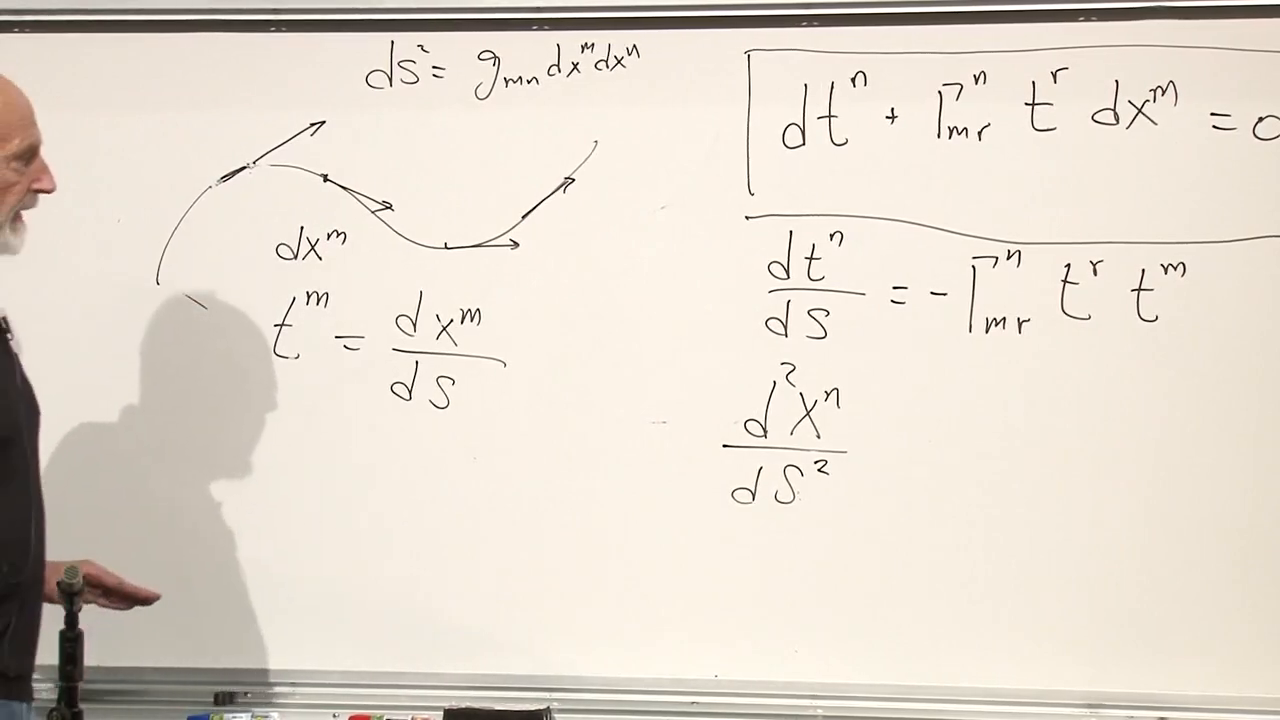
\includegraphics[width=0.94\textwidth]{lecture_04_figure_11.png}
\caption{切矢量移动律与二阶测地线方程。}
\end{figure}

方程\eqref{eq:l4-geodesic}已经类似于牛顿动力学。如果把\(s\)替换为适当的时间参数，第一项就是加速度。联络项则像单位质量所受的力，完全由度规决定。在广义相对论中，这个类比成为字面意义：自由粒子沿时空测地线运动，而牛顿所称的引力加速度通过联络显现出来。

\section{从黎曼距离到时空固有时}

讨论现在从弯曲空间转向时空。在惯性笛卡儿坐标中，邻近事件之间的固有时为
\begin{equation}
d\tau^2
=dt^2-dx^2-dy^2-dz^2.
\label{eq:l4-proper-time}
\end{equation}
讲义使用
\begin{equation}
d\tau^2=-g_{\mu\nu}\,dx^\mu dx^\nu
\label{eq:l4-lecture-sign}
\end{equation}
其中
\begin{equation}
g_{\mu\nu}
=
\eta_{\mu\nu}
=
\begin{pmatrix}
-1&0&0&0\\
0&1&0&0\\
0&0&1&0\\
0&0&0&1
\end{pmatrix}.
\label{eq:l4-eta}
\end{equation}
因此，\eqref{eq:l4-lecture-sign}中的外部负号把所选的mostly-plus度规转换为\eqref{eq:l4-proper-time}。坐标为
\begin{equation}
\begin{aligned}
x^\mu&=(t,x,y,z),\\
x^0&=t,\quad x^1=x,\\
x^2&=y,\quad x^3=z.
\end{aligned}
\end{equation}

\begin{figure}[htbp]
\centering
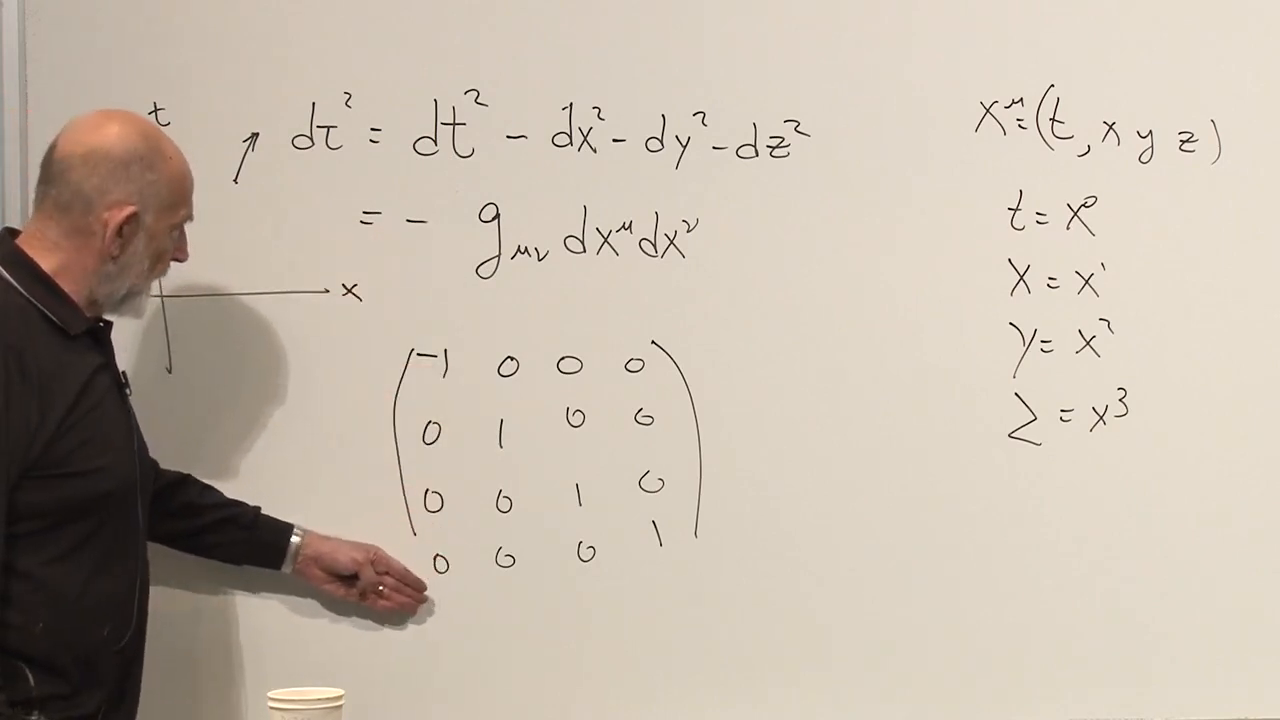
\includegraphics[width=0.94\textwidth]{lecture_04_figure_12.png}
\caption{固有时、时空坐标，以及 mostly-plus 的闵可夫斯基度规。}
\end{figure}

号差才是其不变的信息：一个本征值具有与时间相联系的符号，三个具有与空间相联系的符号。将整个度规乘以 \(-1\) 并相应地调整每一个约定，就得到同样常见的 mostly-minus 约定。没有任何物理内容依赖于这一整体选择。

讲座中问到，是否考虑过具有其他不定号差的空间。在数学上，具有多种号差的伪黎曼几何早已确立。物理上的要点则更为狭窄：观测到的相对论时空是洛伦兹型的，只有一个时间方向。额外的时间性方向会深刻改变因果结构，并且不能描述这里所讨论的物理。

\begin{figure}[htbp]
\centering
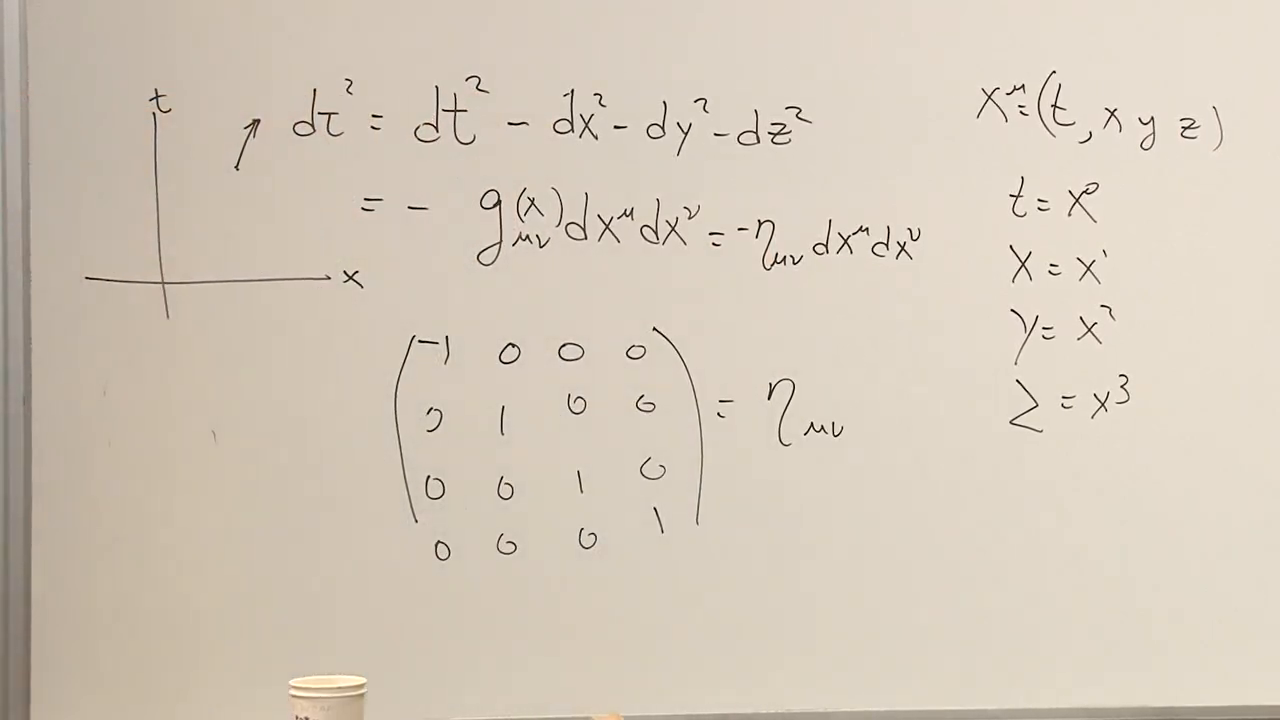
\includegraphics[width=0.94\textwidth]{lecture_04_figure_13.png}
\caption{在用 \(\eta_{\mu\nu}\) 表示平直度规之前，先检查符号约定。}
\end{figure}

平直时空并不意味着度规分量在每一个坐标系中都必定看起来像 \(\eta_{\mu\nu}\)。它的意思是，存在某些坐标系使它们如此。即使黎曼张量为零，曲线坐标或加速坐标也可以使分量随位置变化。

\section{为什么相等的坐标加速度并不刚性}

我们想要附着在一个加速电梯上的坐标。第一个想法是把一组观察者按固定间隔排成一列，并赋予他们全都相同的坐标加速度。相对论使这一朴素构造无法保持刚性。

\begin{figure}[htbp]
\centering
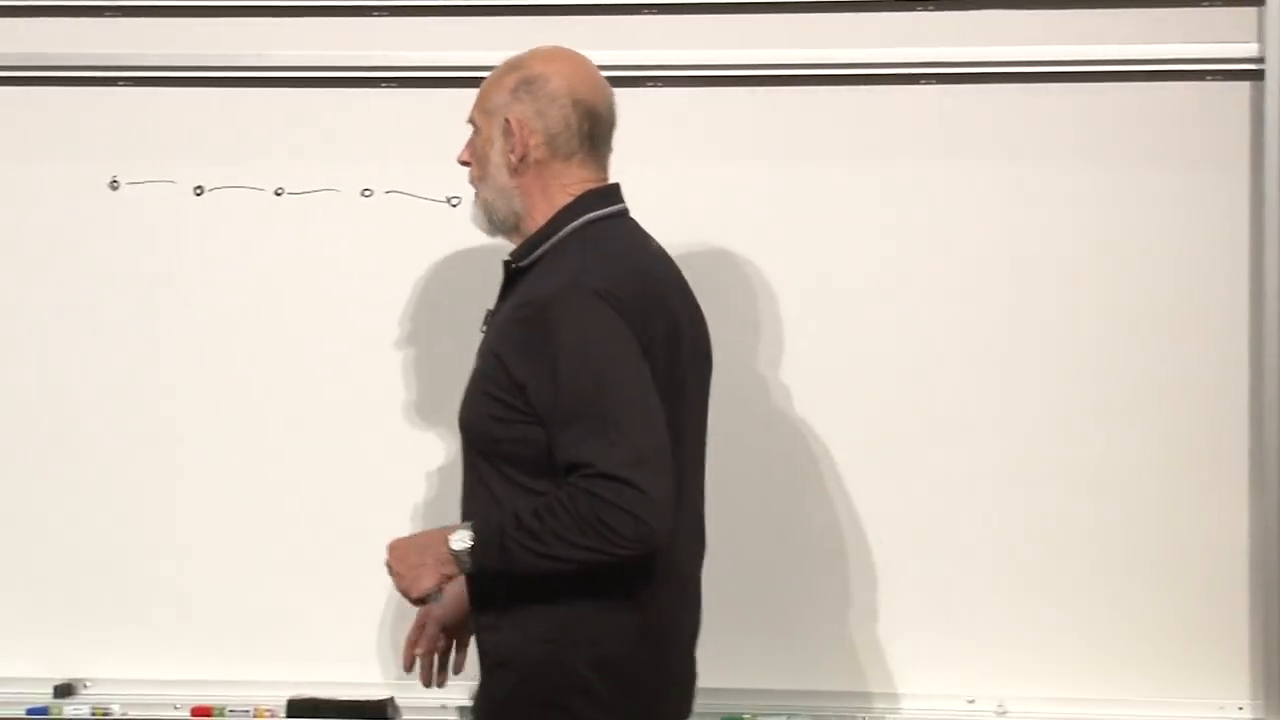
\includegraphics[width=0.92\textwidth]{lecture_04_figure_14.png}
\caption{一列相邻的观察者，用来检验共同的加速度是否保持刚性。}
\end{figure}

如果彼此分开的观察者按照某个惯性系来看遵循相同的加速方案，那么在他们不断变化的瞬时静止系中，他们之间的距离并不会保持固定。连接他们的绳子会被拉伸，并最终断裂。这正是贝尔飞船思想实验所表现出的同一种运动学张力。此外，恒定的牛顿坐标加速度不可能无限持续下去：它最终会预言出大于光速的速率。

因此，相对论性刚性的加速参考系必须在每个位置使用不同的固有加速度。越靠近那个将成为视界的位置的观察者，加速得越强；越远的观察者，加速得越缓。这样，他们的固有间隔就可以在瞬时共动系中保持恒定。这就是一维空间中的玻恩刚性加速。

\section{作为热身练习的欧几里得极坐标}

从普通的圆开始，最容易看清正确的构造。在欧几里得平面中，
\begin{equation}
x=r\cos\theta,
\qquad
y=r\sin\theta,
\end{equation}
所以
\begin{equation}
x^2+y^2=r^2,
\qquad
\cos^2\theta+\sin^2\theta=1.
\end{equation}
复指数形式为
\begin{equation}
\cos\theta=\frac{e^{i\theta}+e^{-i\theta}}{2},
\qquad
\sin\theta=\frac{e^{i\theta}-e^{-i\theta}}{2i}.
\label{eq:l4-euler-trig}
\end{equation}
正弦公式分母中的 \(i\) 因子在课堂讨论中被发现并补回。

\begin{figure}[htbp]
\centering
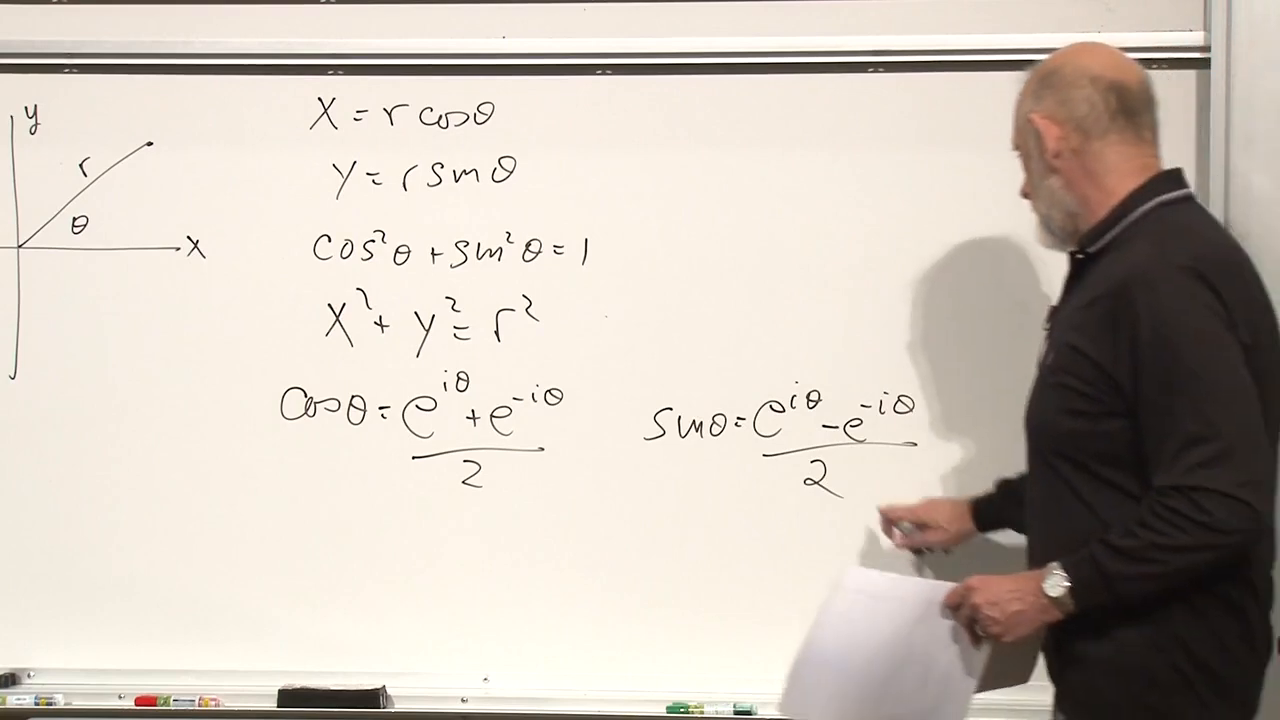
\includegraphics[width=0.94\textwidth]{lecture_04_figure_15.png}
\caption{圆、欧几里得极坐标及其指数三角函数形式。}
\end{figure}

\(r\) 的固定值是一条圆。具有恒定角速率的运动具有大小恒定的向心加速度，方向始终向内。双曲线将在时空中扮演相应的角色。

\section{闵可夫斯基时空中的双曲坐标}

把三角函数替换为它们的双曲对应物：
\begin{equation}
\cosh\omega=\frac{e^\omega+e^{-\omega}}{2},
\qquad
\sinh\omega=\frac{e^\omega-e^{-\omega}}{2},
\end{equation}
其中
\begin{equation}
\cosh^2\omega-\sinh^2\omega=1.
\label{eq:l4-hyperbolic-identity}
\end{equation}
这里没有 \(i\) 因子。坐标 \(\omega\) 是一个双曲角，或称快度。与普通角度不同，它不是周期性的；它的取值范围从 \(-\infty\) 到 \(+\infty\)。

\begin{figure}[htbp]
\centering
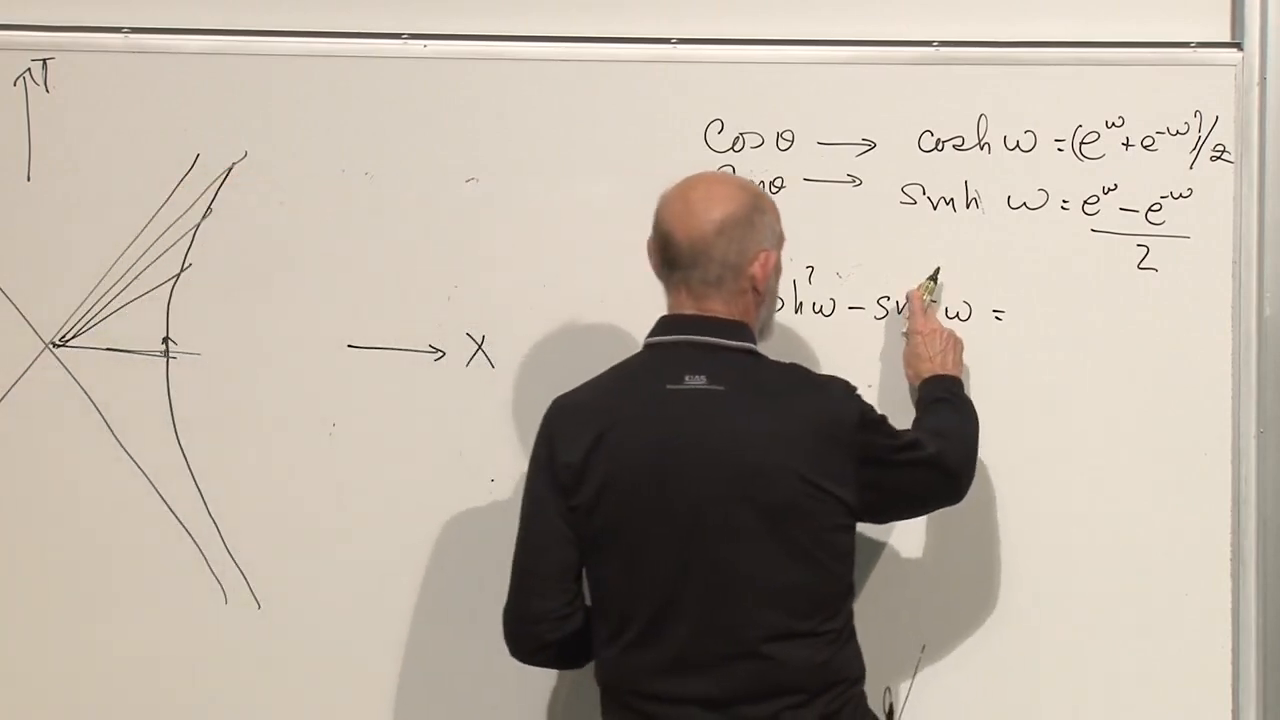
\includegraphics[width=0.94\textwidth]{lecture_04_figure_16.png}
\caption{在时空构造中，圆函数被双曲函数所取代。}
\end{figure}

在右林德勒楔形中定义新坐标：
\begin{equation}
x=r\cosh\omega,
\qquad
t=r\sinh\omega,
\qquad
r>0.
\label{eq:l4-rindler-transform}
\end{equation}
于是
\begin{equation}
x^2-t^2=r^2.
\label{eq:l4-rindler-hyperbola}
\end{equation}
在 \(r\) 固定时，改变 \(\omega\) 描出一条双曲线。增大 \(r\) 会以类空方向穿过这一族双曲线，而增大 \(\omega\) 则沿着其中一条双曲线以类时方向向前移动。

\begin{figure}[htbp]
\centering
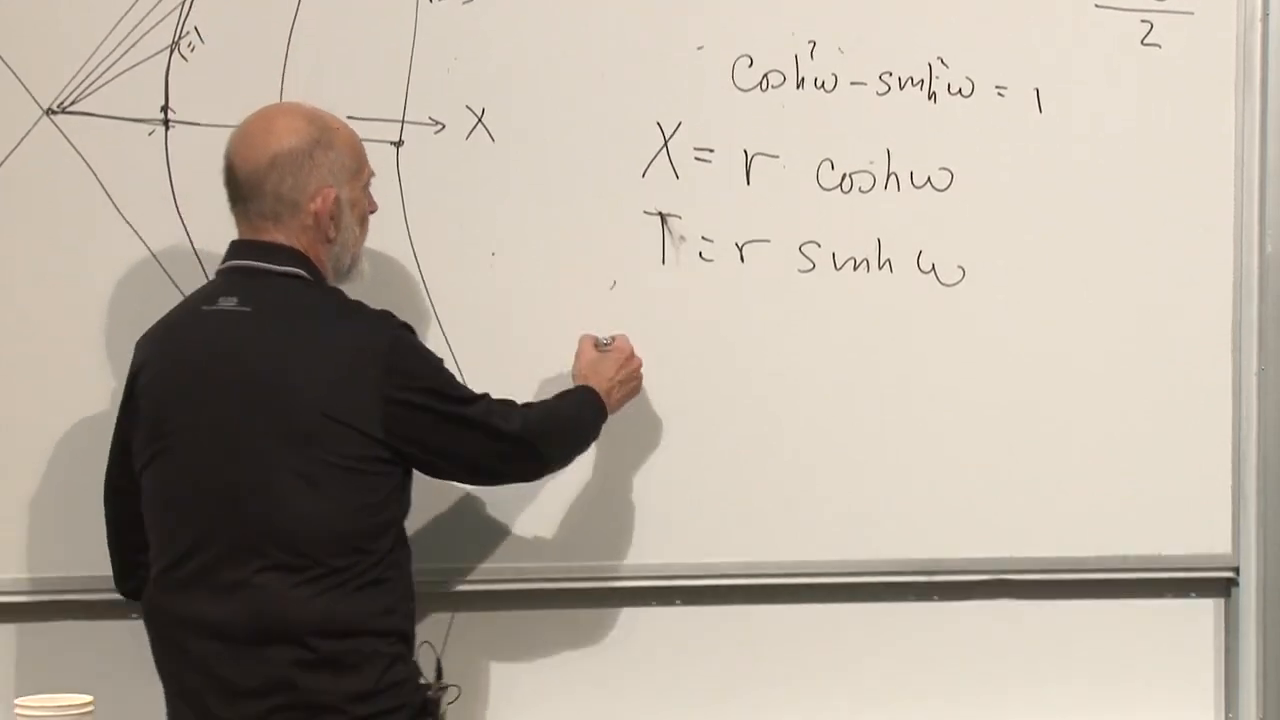
\includegraphics[width=0.94\textwidth]{lecture_04_figure_17.png}
\caption{坐标变换 \(x=r\cosh\omega\)、\(t=r\sinh\omega\) 及其不变双曲线。}
\end{figure}

\begin{figure}[htbp]
\centering
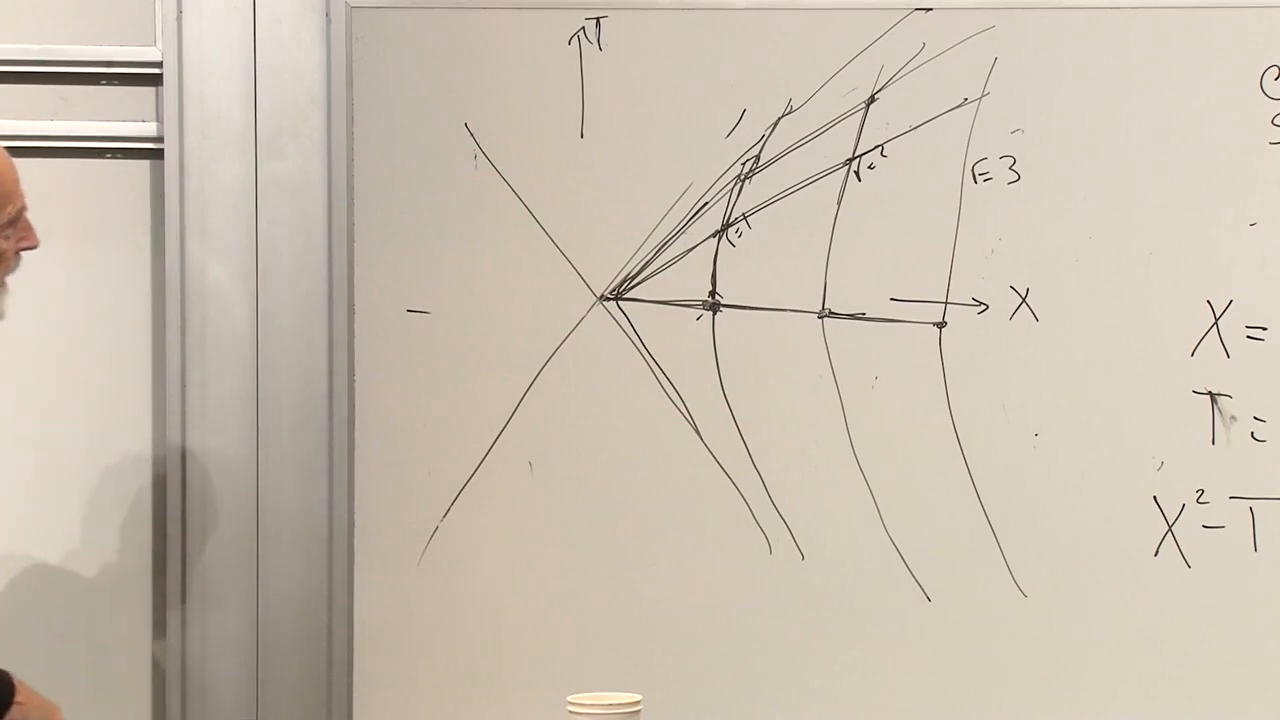
\includegraphics[width=0.94\textwidth]{lecture_04_figure_18.png}
\caption{一族固定 \(r\) 的双曲线，表示一个刚性加速的观察者族。}
\end{figure}

\subsection{加速坐标中的度规}

对 \eqref{eq:l4-rindler-transform} 求微分：
\begin{align}
dx&=\cosh\omega\,dr+r\sinh\omega\,d\omega,\\
dt&=\sinh\omega\,dr+r\cosh\omega\,d\omega.
\end{align}
利用 \eqref{eq:l4-hyperbolic-identity}，交叉项相消：
\begin{align}
d\tau^2
&=dt^2-dx^2\\
&=r^2\,d\omega^2-dr^2.
\label{eq:l4-rindler-metric}
\end{align}
当横向方向被恢复时，只需在此处所用的固有时约定中加上 \(-dy^2-dz^2\)。

这仍然是平直时空。依赖于坐标的系数\(r^2\)并不比欧几里得极坐标中乘在\(d\theta^2\)上的\(r^2\)更能说明存在曲率。

\subsection{双曲线上的固有加速度}

对于一条固定的世界线\(r=R\)，方程\eqref{eq:l4-rindler-metric}给出
\begin{equation}
d\tau=R\,d\omega.
\end{equation}
其四维速度为
\begin{equation}
U^\mu
=
\frac{d(t,x)}{d\tau}
=
(\cosh\omega,\sinh\omega),
\end{equation}
而其四维加速度为
\begin{equation}
A^\mu
=
\frac{dU^\mu}{d\tau}
=
\frac{1}{R}(\sinh\omega,\cosh\omega).
\end{equation}
其不变量的大小是常数：
\begin{equation}
a=\sqrt{A^\mu A_\mu}=\frac{1}{R}
\qquad (c=1).
\label{eq:l4-proper-acceleration}
\end{equation}

\begin{figure}[htbp]
\centering
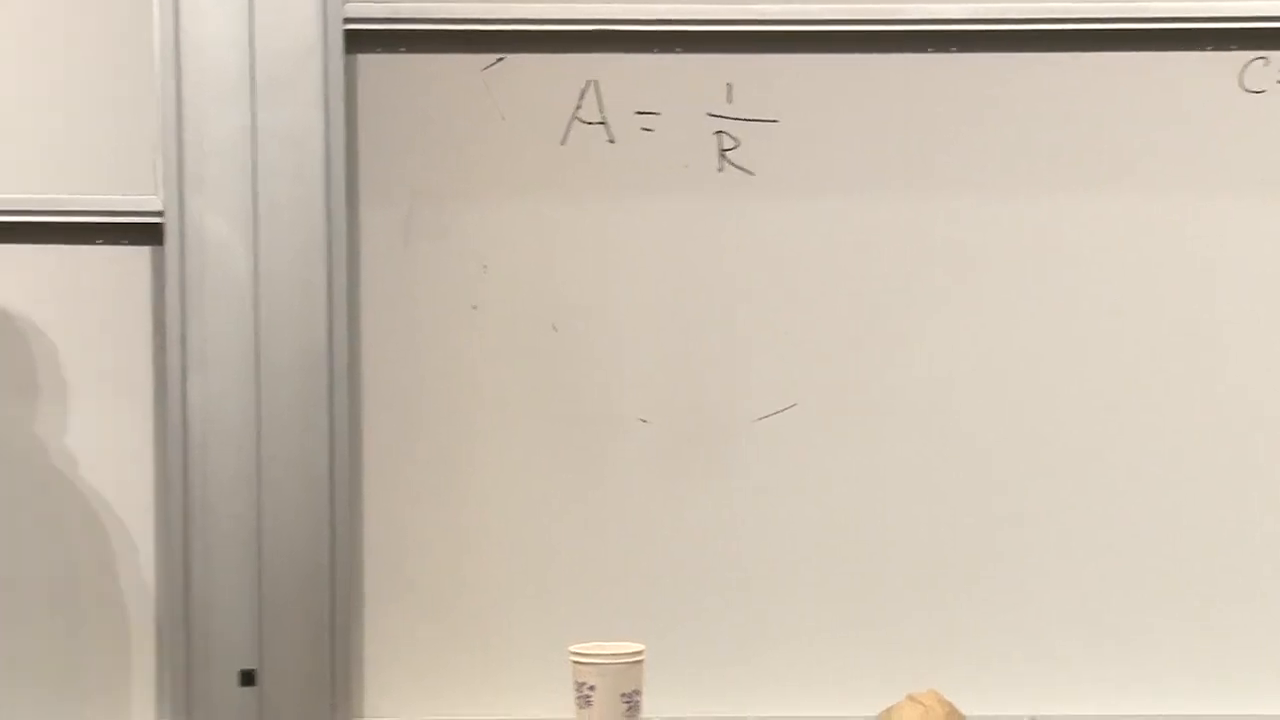
\includegraphics[width=0.90\textwidth]{lecture_04_figure_19.png}
\caption{对于一条固定的加速世界线，反比半径定律\(a=1/R\)。}
\end{figure}

恢复单位后，
\begin{equation}
\boxed{a=\frac{c^2}{R}.}
\label{eq:l4-proper-acceleration-units}
\end{equation}

\begin{figure}[htbp]
\centering
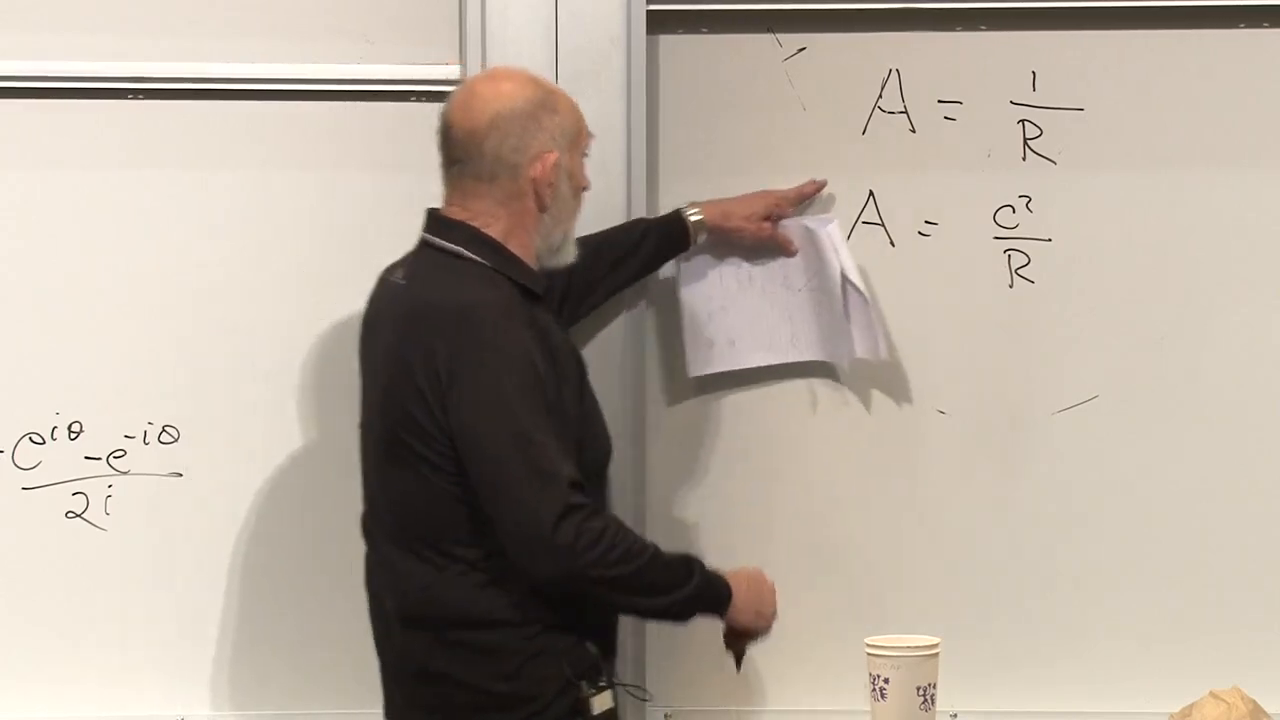
\includegraphics[width=0.90\textwidth]{lecture_04_figure_20.png}
\caption{恢复单位将\(1/R\)转换为\(c^2/R\)。}
\end{figure}

截距\(R\)越小，世界线弯曲得越急剧，其观测者感受到的固有加速度也越大。更远的双曲线弯曲得更少，所需的加速度也更小。每个观测者在时间中都具有恒定的加速度，但不同的观测者具有不同的加速度。正是这种差异保持了它们彼此之间的固有距离。

\subsection{关于加速坐标的问题}

\paragraph{\(R\)是\(x\)截距吗？}
是的。在\(\omega=0\)处，方程\eqref{eq:l4-rindler-transform}给出\(t=0\)和\(x=R\)。该截距通过\eqref{eq:l4-proper-acceleration-units}确定了固有加速度。

\paragraph{这一构造是否依赖于所选取的原点？}
坐标确实如此。平移原点会产生另一族双曲线，其渐近线发生平移。没有任何不变的物理内容依赖于这一选择。我们是在有意选取一个加速坐标系，并追问惯性运动在用它来描述时呈现为何种样子。

\paragraph{什么是固有加速度？}
它是观测者随身携带的加速度计所测得的加速度。用协变方式表示，
\begin{equation}
A^\mu=\frac{dU^\mu}{d\tau},
\qquad
U^\mu=\frac{dx^\mu}{d\tau}.
\end{equation}
其大小是观测者实际感受到的推力，而不是由遥远参考系所指定的坐标加速度\(d^2x/dt^2\)。

\section{极坐标与双曲坐标中的平直度规}

在靠近地球进行局部化之前，把欧几里得度规与洛伦兹度规并排放在一起是有益的。在平面中，
\begin{equation}
ds^2=dr^2+r^2d\theta^2,
\qquad
g_{ab}
=
\begin{pmatrix}
1&0\\
0&r^2
\end{pmatrix}.
\label{eq:l4-polar-metric}
\end{equation}
听众的一个建议短暂地引入了一个球面因子，但这只是一个平面，而不是一个球面。\(r^2\)项记录了这一事实：固定的角间隔在更大的半径处张成更长的弧。

\begin{figure}[htbp]
\centering
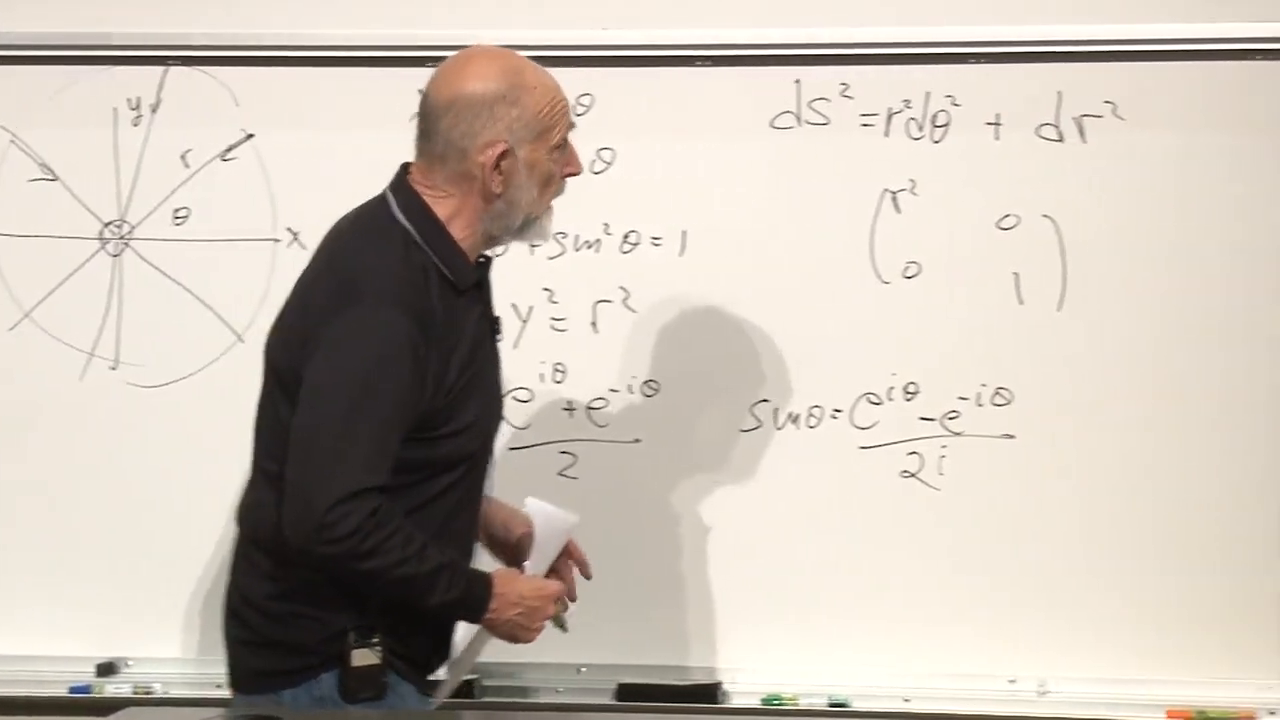
\includegraphics[width=0.94\textwidth]{lecture_04_figure_21.png}
\caption{欧几里得极坐标度规：平直平面中依赖于位置的各分量。}
\end{figure}

闵可夫斯基的对应物是
\begin{equation}
d\tau^2=r^2d\omega^2-dr^2.
\end{equation}
两个度规都具有依赖于位置的分量，然而两种几何都是平直的。坐标曲率与几何曲率并不是同一回事。

\section{在地面加速度附近进行局部化}

选取一条参考双曲线，其固有加速度为地面值\(g\)：
\begin{equation}
g=\frac{c^2}{R},
\qquad
R=\frac{c^2}{g}.
\label{eq:l4-earth-radius}
\end{equation}

\begin{figure}[htbp]
\centering
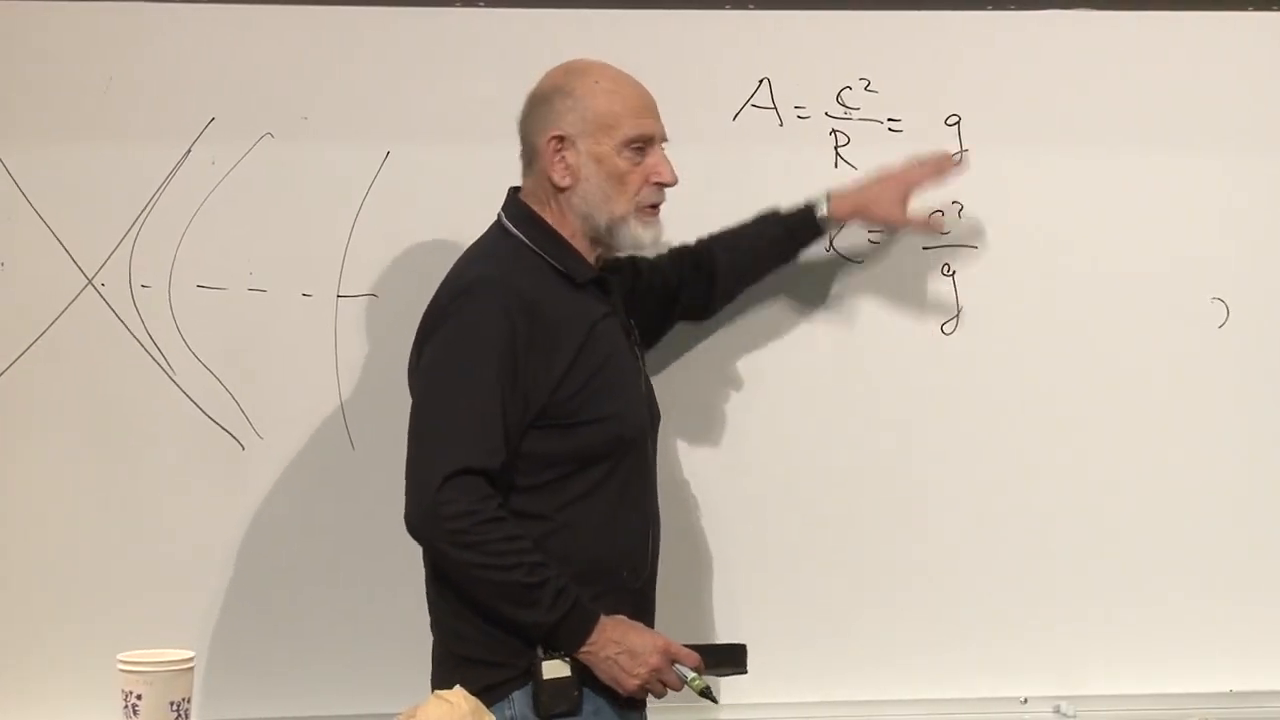
\includegraphics[width=0.94\textwidth]{lecture_04_figure_22.png}
\caption{通过\(c^2/R=g\)选取参考双曲线。}
\end{figure}

数值上，
\begin{equation}
R
\simeq
\frac{(3.0\times10^8\ {\rm m\,s^{-1}})^2}
{9.8\ {\rm m\,s^{-2}}}
\simeq
9.2\times10^{15}\ {\rm m}.
\end{equation}
讲座将其取整为\(10^{16}\)米。一个地面\(g\)的场在相对论尺度上是微不足道的，因此相应的林德勒半径极其巨大。

现在只考察该参考观测者的一个小邻域。通过下式引入局部高度\(y\)
\begin{equation}
r=R+y,
\qquad
dr=dy,
\qquad
|y|\ll R.
\label{eq:l4-local-height}
\end{equation}
等式\(dr=dy\)在讨论中被明确地捕捉到，因此空间项必须写成\(-dy^2\)。

代入\eqref{eq:l4-rindler-metric}得到
\begin{align}
d\tau^2
&=(R+y)^2d\omega^2-dy^2\\
&=(R^2+2Ry+y^2)d\omega^2-dy^2\\
&=
\left(
1+\frac{2y}{R}+\frac{y^2}{R^2}
\right)
R^2d\omega^2-dy^2.
\label{eq:l4-local-expand}
\end{align}

\begin{figure}[htbp]
\centering
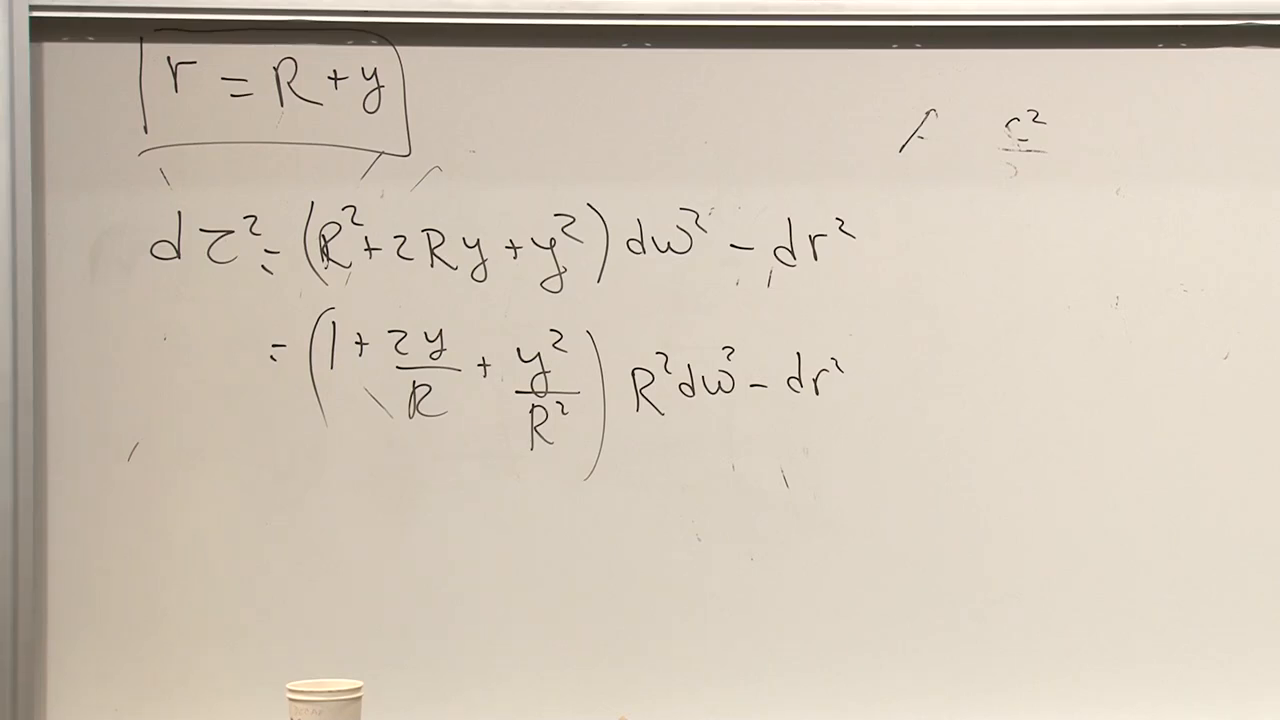
\includegraphics[width=0.94\textwidth]{lecture_04_figure_23.png}
\caption{在\(r=R+y\)附近展开加速度规。}
\end{figure}

定义局部时间坐标
\begin{equation}
t=R\omega.
\label{eq:l4-local-time}
\end{equation}
于是
\begin{equation}
d\tau^2
=
\left(
1+\frac{2y}{R}+\frac{y^2}{R^2}
\right)dt^2-dy^2.
\label{eq:l4-local-exact}
\end{equation}

\begin{figure}[htbp]
\centering
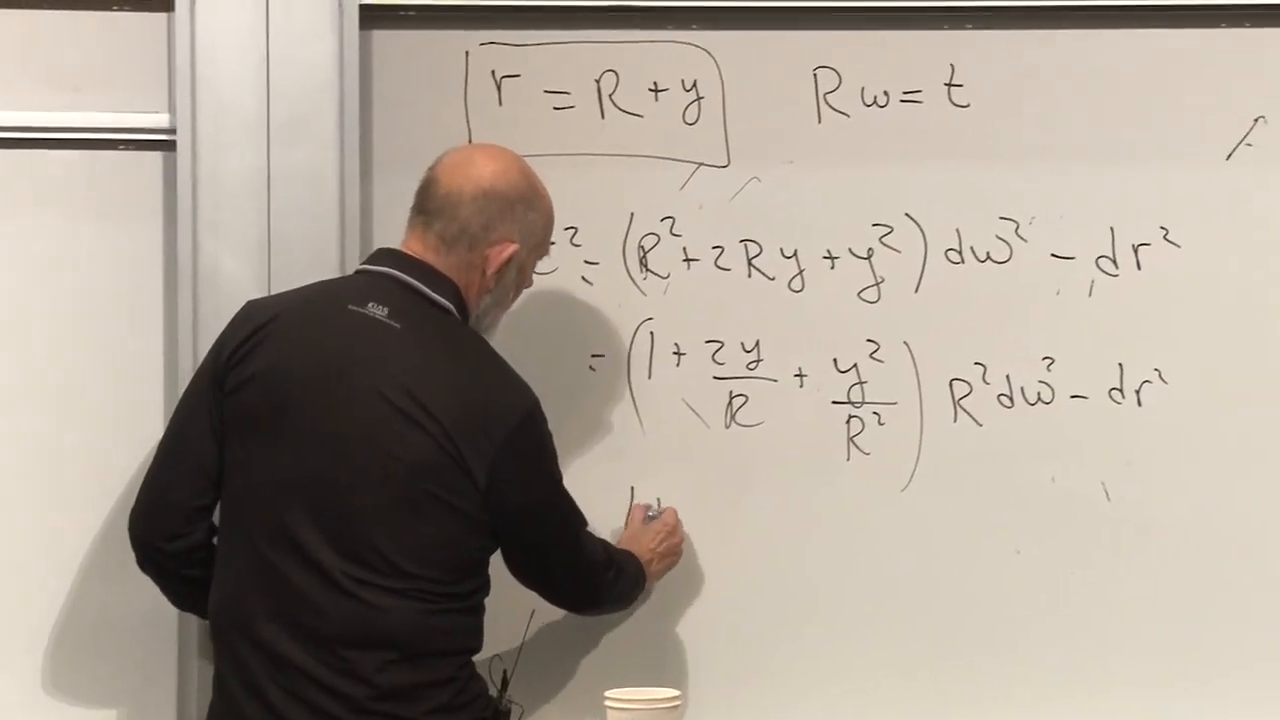
\includegraphics[width=0.94\textwidth]{lecture_04_figure_24.png}
\caption{在参考双曲线附近展开之后引入\(t=R\omega\)。}
\end{figure}

即使几十千米的竖直偏移，与\(R\)相比也是微小的。讲座用大约二十四英里的下落来使这一比较变得生动：这样的距离与\(10^{16}\)米相比仍然可以忽略。因此\(y^2/R^2\)远小于\(y/R\)，二次项可以略去：
\begin{equation}
d\tau^2
\simeq
\left(1+\frac{2y}{R}\right)dt^2-dy^2.
\label{eq:l4-local-linear}
\end{equation}

\begin{figure}[htbp]
\centering
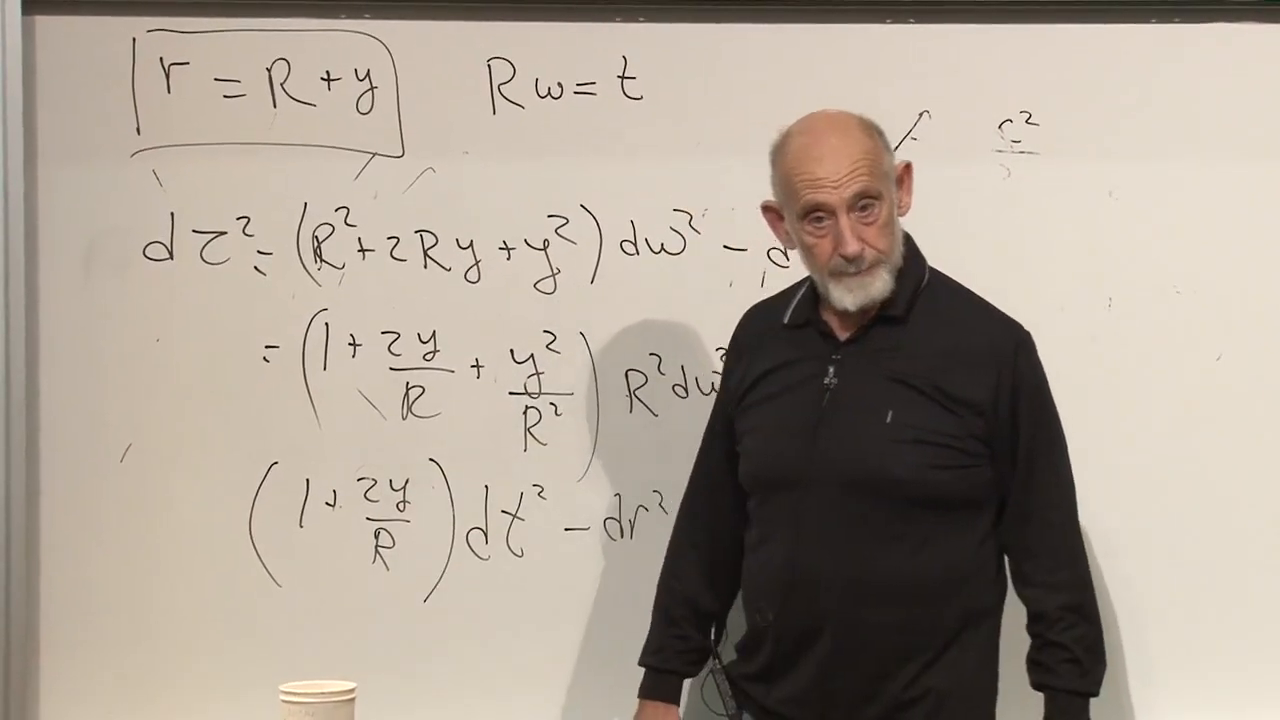
\includegraphics[width=0.94\textwidth]{lecture_04_figure_25.png}
\caption{弱场截断之前的展开度规与局部时间代换。}
\end{figure}

在\(c=1\)的单位制下，方程\eqref{eq:l4-earth-radius}给出\(1/R=g\)，因此
\begin{equation}
\boxed{
d\tau^2\simeq(1+2gy)\,dt^2-dy^2.
}
\label{eq:l4-uniform-metric}
\end{equation}

\begin{figure}[htbp]
\centering
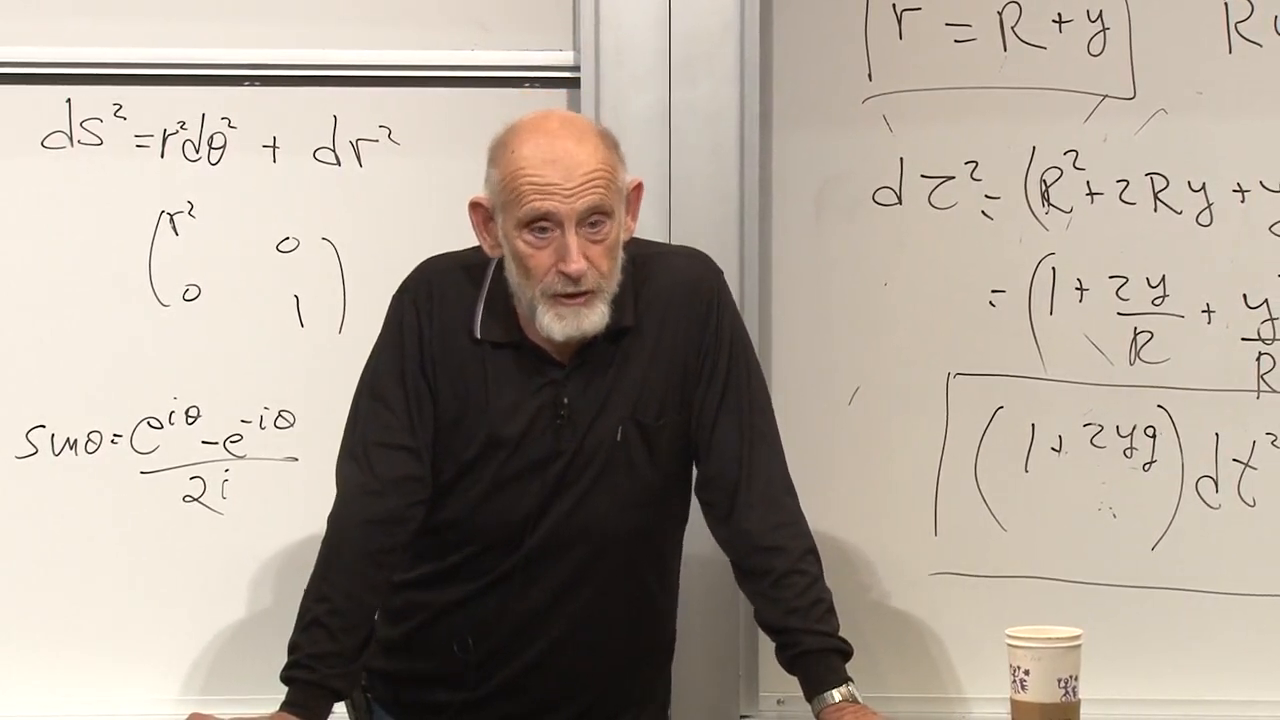
\includegraphics[width=0.94\textwidth]{lecture_04_figure_26.png}
\caption{均匀加速升降机的完整局部度规。}
\end{figure}

量
\begin{equation}
\Phi(y)=gy
\end{equation}
是均匀场中单位质量的牛顿引力势。因此
\begin{equation}
d\tau^2\simeq(1+2\Phi)\,dt^2-dy^2
\qquad (c=1).
\label{eq:l4-weak-potential-propertime}
\end{equation}
按照讲座的约定\(d\tau^2=-g_{\mu\nu}dx^\mu dx^\nu\)，这意味着
\begin{equation}
g_{tt}=-(1+2\Phi).
\label{eq:l4-gtt-potential}
\end{equation}
在常规单位下，无量纲修正为\(2\Phi/c^2\)。

没有任何东西使时空弯曲。方程\eqref{eq:l4-uniform-metric}是平坦的Rindler度规的局部展开。其表观引力是在加速升降机内部看到的惯性力。

\section{测地线方程变为牛顿定律}

将\(gy\)等同于势，迄今为止只是暗示性的。决定性的检验是动力学上的：度规\eqref{eq:l4-uniform-metric}中的自由粒子是否以\(d^2y/dt^2=-g\)向下加速？

对于以固有时参数化的类时世界线，
\begin{equation}
\frac{d^2x^\nu}{d\tau^2}
+\Gamma^\nu{}_{\mu\rho}
\frac{dx^\mu}{d\tau}
\frac{dx^\rho}{d\tau}
=0.
\label{eq:l4-spacetime-geodesic}
\end{equation}
其竖直分量为
\begin{equation}
\frac{d^2y}{d\tau^2}
=
-\Gamma^y{}_{\mu\rho}
\frac{dx^\mu}{d\tau}
\frac{dx^\rho}{d\tau}.
\label{eq:l4-y-geodesic}
\end{equation}

\begin{figure}[htbp]
\centering
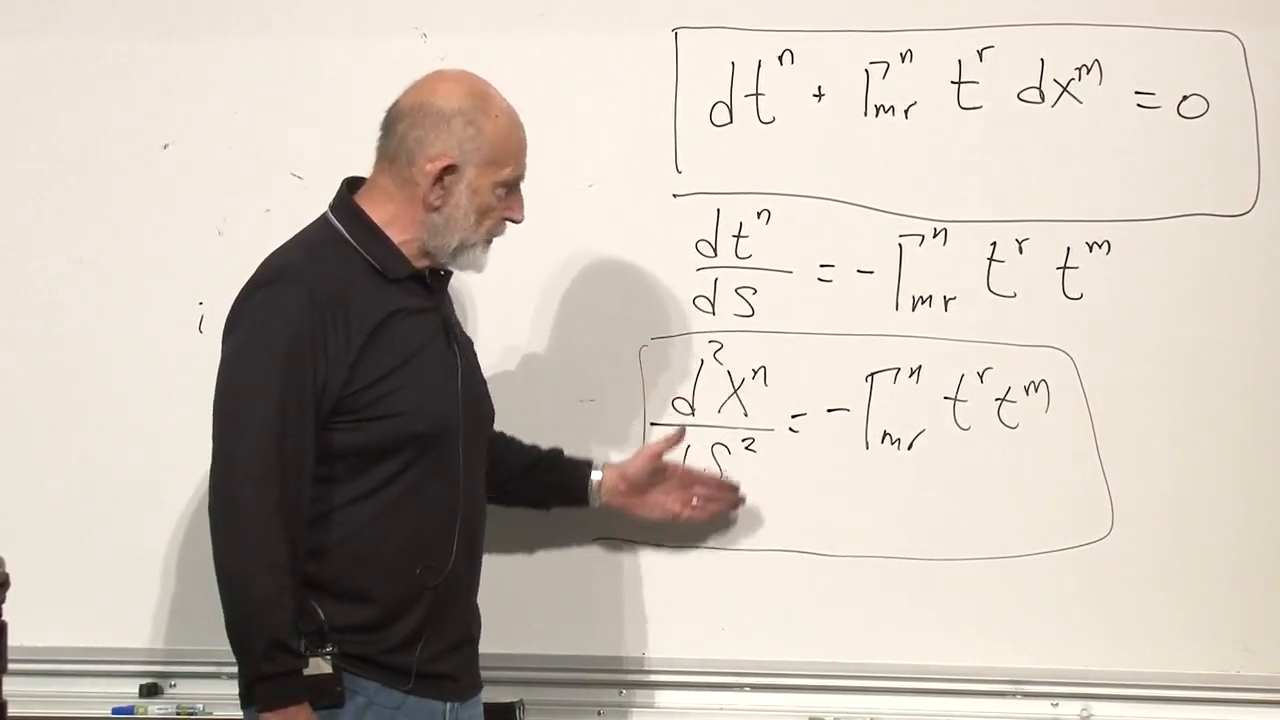
\includegraphics[width=0.94\textwidth]{lecture_04_figure_27.png}
\caption{输运方程及其二阶测地线形式，已准备好应用于竖直运动。}
\end{figure}

\subsection{慢运动近似}

对于弱静态场中缓慢运动的粒子，
\begin{equation}
\frac{dt}{d\tau}\simeq1,
\qquad
\left|\frac{dy}{d\tau}\right|\ll1.
\end{equation}
因此四维速度的时间分量为1阶，而空间分量与之相比很小。在\eqref{eq:l4-y-geodesic}中的乘积里，占主导的一项具有\(\mu=\rho=t\)：
\begin{equation}
\frac{d^2y}{d\tau^2}
\simeq
-\Gamma^y{}_{tt}
\left(\frac{dt}{d\tau}\right)^2
\simeq
-\Gamma^y{}_{tt}.
\label{eq:l4-slow-geodesic}
\end{equation}

\begin{figure}[htbp]
\centering
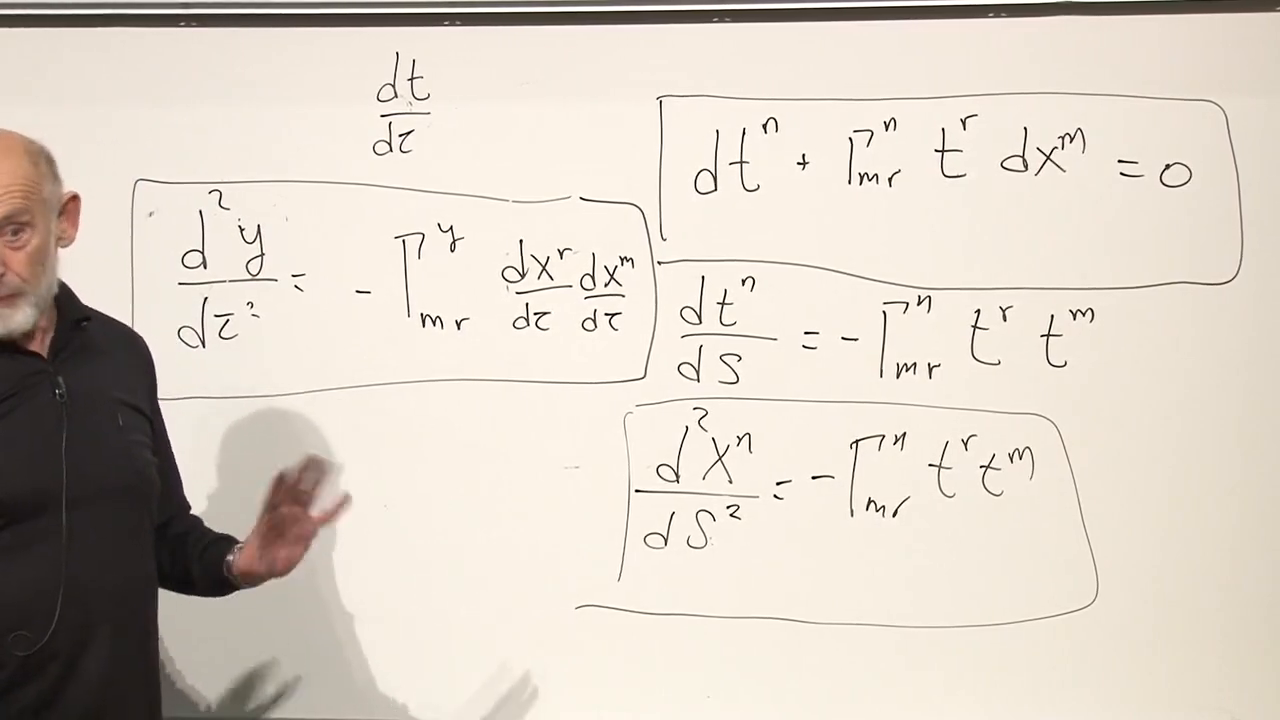
\includegraphics[width=0.94\textwidth]{lecture_04_figure_28.png}
\caption{将时空测地线方程特殊化到缓慢运动的\(y\)分量。}
\end{figure}

现在计算所需的一个联络系数。度规是对角的且与\(t\)无关，所以
\begin{align}
\Gamma^y{}_{tt}
&=
\frac{1}{2}g^{yy}
\left(
\partial_tg_{yt}
+\partial_tg_{ty}
-\partial_yg_{tt}
\right)\\
&=
-\frac{1}{2}\partial_yg_{tt},
\label{eq:l4-gamma-ytt}
\end{align}
因为在本讲义的主要为正号的张量约定中\(g^{yy}=1\)。

\begin{figure}[htbp]
\centering
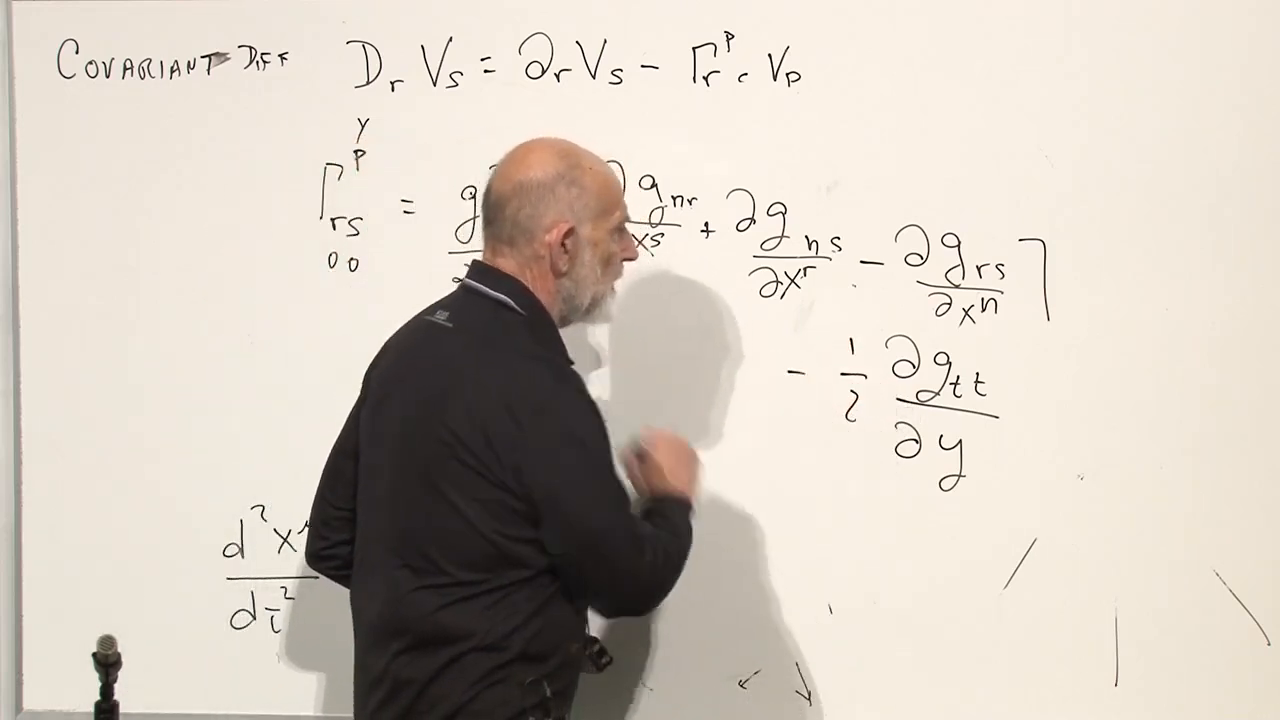
\includegraphics[width=0.94\textwidth]{lecture_04_figure_29.png}
\caption{Christoffel公式化简到\(y,t,t\)分量。}
\end{figure}

结合\eqref{eq:l4-slow-geodesic}与\eqref{eq:l4-gamma-ytt}，
\begin{equation}
\frac{d^2y}{d\tau^2}
\simeq
\frac{1}{2}\partial_yg_{tt}.
\label{eq:l4-accel-gtt}
\end{equation}
由\eqref{eq:l4-gtt-potential}，
\begin{equation}
\partial_yg_{tt}
=
-2\partial_y\Phi
=
-2g.
\end{equation}
因此
\begin{equation}
\boxed{
\frac{d^2y}{d\tau^2}=-g.
}
\label{eq:l4-newton-result}
\end{equation}
由于在同一慢运动近似中\(t\simeq\tau\)，这也就是
\begin{equation}
\frac{d^2y}{dt^2}=-g.
\end{equation}

\begin{figure}[htbp]
\centering
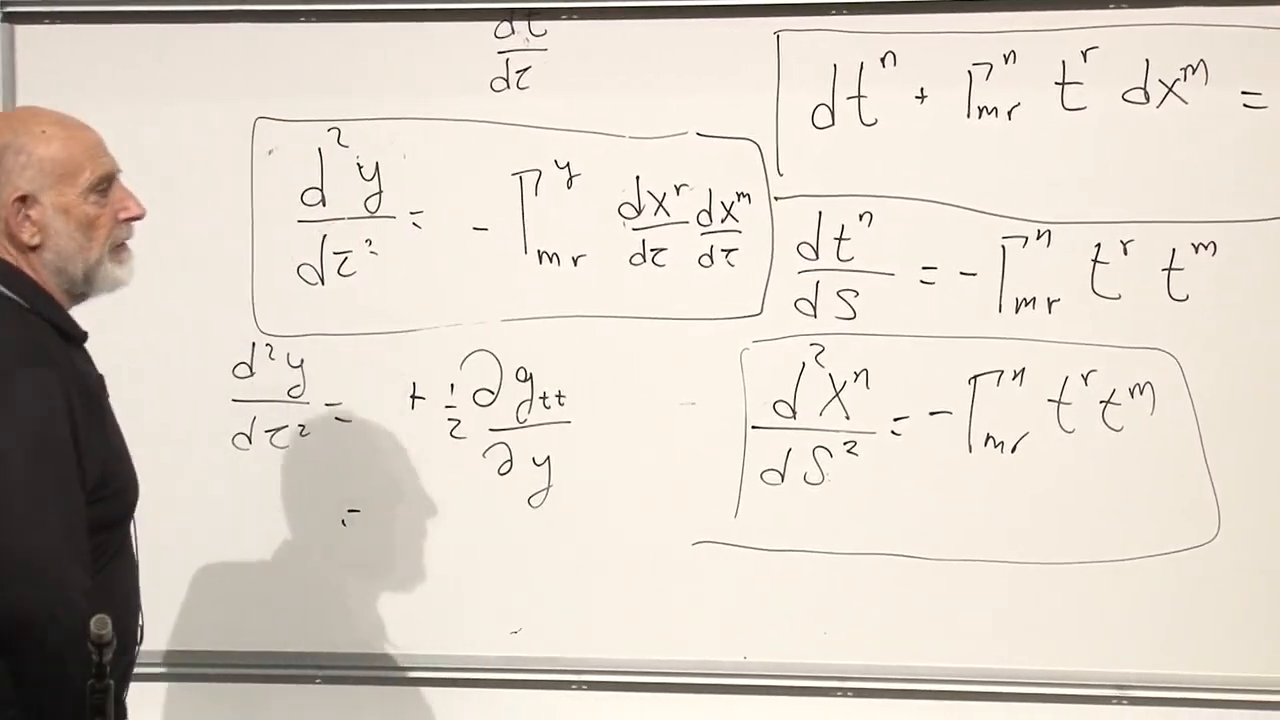
\includegraphics[width=0.94\textwidth]{lecture_04_figure_30.png}
\caption{完整的符号链：\(g_{tt}\)的\(y\)导数产生加速度\(-g\)。}
\end{figure}

更一般地，在牛顿区域中，
\begin{equation}
\boxed{
\begin{aligned}
g_{tt}&=-(1+2\Phi),\\
\frac{d^2x^i}{dt^2}&=-\partial_i\Phi
\end{aligned}
}
\qquad(c=1).
\label{eq:l4-newton-general}
\end{equation}
恢复单位后，度规修正为\(2\Phi/c^2\)，而加速度仍为\(-\boldsymbol{\nabla}\Phi\)。

这一计算解释了为什么度规，而非单独的引力场，才是核心对象。自由粒子只是沿时空测地线运动。在适应于加速实验室的坐标中，该测地线具有通常被归因于引力的坐标曲率。

\subsection{关于所选Rindler原点的问题}

参考双曲线能否被平移，使其渐近线和截距出现在别处？可以。对于每一个合适的平移原点，都存在一个相应的匀加速坐标系。在升降机图像中，这些选择相当于选取其地板在某一瞬间占据不同位置的升降机。

局部结果并不依赖于某个享有特权的原点。一旦选定了加速度为\(g\)的参考观测者，\(y\)就测量相对于该观测者的高度，而附近的度规取形式\eqref{eq:l4-uniform-metric}。任意的坐标选择决定我们在哪里描述地板；它并不产生不变曲率。

\section{为什么Christoffel符号不能是张量}

课后讨论回到一个在复习中首次出现的要点。在原来的惯性坐标中，
\begin{equation}
g_{\mu\nu}=\eta_{\mu\nu},
\qquad
\partial_\rho\eta_{\mu\nu}=0,
\qquad
\Gamma^\mu{}_{\nu\rho}=0.
\end{equation}
自由粒子沿直线运动，不存在引力。

在加速坐标中，同一平坦时空具有依赖于位置的度规分量。其Christoffel符号不为零，而同一条惯性轨迹看起来是弯曲的。粒子似乎朝着升降机的地板下落。

如果\(\Gamma^\mu{}_{\nu\rho}\)是张量，这就不可能。在一个参考系中为零的张量在每个参考系中都为零。相反，联络在坐标变换下获得一个非齐次项，因此它可以在惯性系中为零，而在加速系中不为零。这正是等效原理所要求的：
\begin{equation}
\text{accelerated frame}
\quad\longleftrightarrow\quad
\text{local gravity}.
\end{equation}

曲率的表现不同。Riemann张量是张量。如果它在惯性系中为零，那么它在加速系中也同样为零：
\begin{equation}
R^\mu{}_{\nu\rho\sigma}=0.
\end{equation}
因此，Christoffel符号描述依赖于坐标的引力，而曲率探测的是任何坐标改变都无法去除的不变潮汐内容。

\section{从均匀势到Schwarzschild预览}

加速升降机没有引力物质，也没有曲率。然而，弱场关系\eqref{eq:l4-newton-general}暗示了在实际球对称质量场中应当寻找什么。质量\(M\)外部的牛顿势为
\begin{equation}
\Phi(r)=-\frac{GM}{r}.
\label{eq:l4-newton-potential}
\end{equation}
将其代入弱场时间分量得到
\begin{equation}
g_{tt}
\simeq
-\left(1-\frac{2GM}{r}\right)
\qquad(c=1).
\label{eq:l4-schwarzschild-preview}
\end{equation}
势的符号在板书讨论中得到修正。吸引要求一个负势，当\(r\)趋于无穷时它从下方趋于零。

\begin{figure}[htbp]
\centering
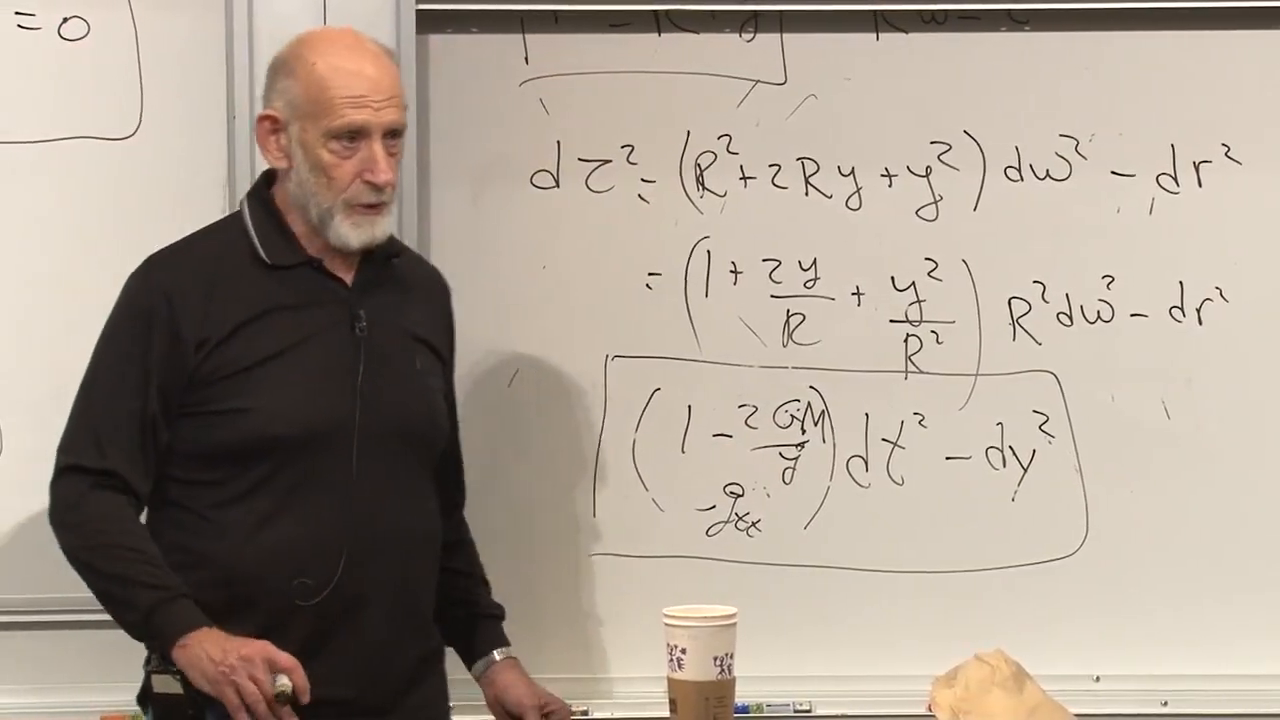
\includegraphics[width=0.94\textwidth]{lecture_04_figure_31.png}
\caption{将牛顿势代入时间-时间度规系数，即可看出因子\(1-2GM/r\)。}
\end{figure}

该系数在
\begin{equation}
r=2GM
\qquad(c=1),
\end{equation}
处为零，或者，恢复单位后，
\begin{equation}
r_s=\frac{2GM}{c^2}.
\end{equation}
这就是施瓦西半径。这个特定度规系数的消失预示着一个视界。

这一论证是特意作为预览而非推导给出的。仅靠弱场近似无法确立\(r=2GM/c^2\)附近的精确施瓦西解，而那里恰恰是修正不再微小之处。完整解还包含一个非平凡的径向分量，并且必须满足爱因斯坦场方程。那些方程尚未引入。目前的推理所揭示的是正确的结构性线索，以及某种定性上全新的现象必然出现的尺度。

\section{课堂问题与更正}

\subsection{双曲角的行为像普通角吗？}

不。二者都参数化沿一族等半径曲线的运动，但\(\theta\)是周期的，而快度\(\omega\)取遍实直线。角这个词指的是旋转与洛伦兹助推之间的代数类比，而不是指一个被限制在\(0\)与\(2\pi\)之间的量。

\subsection{为什么一个不大的加速度需要巨大的R？}

关系式\(a=c^2/R\)包含巨大的相对论尺度\(c^2\)。要只得到\(10\ {\rm m\,s^{-2}}\)，需要\(R\)的量级为\(10^{16}\)米。这并不是附着于地球的一个新的物理距离。它是闵可夫斯基图中双曲世界线的曲率半径，以长度单位表示。

这个巨大的半径还保证了一个有用的牛顿区间。在实验室的时间和距离尺度上，速度仍远低于\(c\)，加速度在装置各处的变化可忽略不计，并且\(t\)与固有时差别很小。

\subsection{这个表观引力场是真实的吗？}

对于被保持在固定林德勒位置的观测者而言，它作为加速度计读数是真实的，但它不是不变的曲率。释放该观测者，加速度计沿由此产生的惯性测地线读数为零。一个足够小的自由下落实验室可以在局部消除这个均匀场。在一个有限区域内无法消除的是潮汐场，它由非零曲率表示。

\subsection{在力的计算过程中更正了什么？}

若干符号和一个二分之一因子被当场核对。在讲座的约定下，可靠的链条是
\begin{equation}
\begin{aligned}
g_{tt}&=-(1+2gy),\\
\Gamma^y{}_{tt}&=-\frac12\partial_yg_{tt}=g,\\
\frac{d^2y}{d\tau^2}&=-\Gamma^y{}_{tt}=-g.
\end{aligned}
\end{equation}
明确写出约定可以防止板书层面的符号犹豫变成物理上的歧义。

\section{已经确立的内容}

讲座从微分几何开始，以牛顿的下落物体结束。关键步骤如下：
\begin{enumerate}
\item 协变导数在变化的坐标基中比较张量。
\item 平行移动意味着沿选定路径的协变变化为零。
\item 测地线平行移动自身的切向量。
\item 自由粒子沿时空的测地线运动。
\item 固定\(r\)的双曲线构成一个相对论性刚性的加速参考系。
\item 它们的固有加速度为\(a=c^2/r\)，因此它必须随位置变化。
\item 在加速度为\(g\)的参考世界线附近，平直度规为
\begin{equation}
d\tau^2\simeq(1+2gy)\,dt^2-dy^2
\qquad(c=1).
\end{equation}
\item 其测地线方程化为
\begin{equation}
\frac{d^2y}{dt^2}=-g.
\end{equation}
\end{enumerate}

因此，等效原理不仅仅是电梯与引力之间的类比。它被编码在度规及其联络的变换方式之中。当平直时空用加速坐标写出时，可以出现一个均匀引力，而曲率仍然为零。

最后的外推指向均匀场之外。将\(\Phi=gy\)替换为\(\Phi=-GM/r\)，可以预言球对称度规时间分量中的特征因子\(1-2GM/r\)，并揭示施瓦西尺度。然而，要确定完整的几何，我们需要场方程。这正是下一讲要转向的任务。
